\documentclass[11pt,a4paper]{article}

\usepackage{fontspec}\setmainfont{Times New Roman}
\usepackage[margin=0.88in]{geometry}
\usepackage{amsmath,amssymb,graphicx,longtable,array,hyperref}\hypersetup{hidelinks}\usepackage{xurl}

\title{Cross-cohort candidate biomarkers in under-served diseases:\\ a transparent multi-disease negative-results study}
\author{MEGA-PROGRAM-27 working analysis}
\date{25 September 2026 - working manuscript; not yet complete}
\begin{document}\maketitle
\begin{abstract}
We evaluate expression-derived gene candidates across ten disease labels (nine with analyzable cohorts), including postpartum depression. A prespecified duplicate-sample audit materially changed earlier apparent replications. In the deduplicated analysis, top-50 signatures passed an empirical-null sign test in polycystic ovary syndrome (PCOS) and interstitial cystitis, though the latter has a small validation cohort; five other testable disease signatures did not pass. A named preeclampsia candidate, GNG2, did not replicate. Independent fresh RNA-seq cohorts falsified the directional ST3GAL2 prediction. A held-out cohort convolutional neural network (CNN) scored below logistic regression on average. The graph neural network (GNN) benchmark is within-project only; no published state-of-the-art comparison or validated new biomarker has yet been established. This manuscript is a working report, not a clinical test claim.
\end{abstract}
\tableofcontents\clearpage
\section{Scope and reproducibility}
The repository contains a runnable Python command-line tool, hermetic tests, result tables, accession manifest, and the source for these figures. The project-level completion gates are not all met: 40 of 40 genuinely used scientific tools, 703 of 120 distinct fetched-and-used accession records, eleven displayed numbered formulas, no externally comparable benchmark break or defensible new named discovery. The 30-page rendered Times working PDF meets a conservative page-level research-content audit: twenty pages each contain at least 250 extracted words of research argument, derivation, methods, findings or limitations, excluding title, contents, sparse tables, tool appendix and references. The page-level test is reproducible in \texttt{scripts/audit\_substantive\_pages.py}; it measures content, not scientific validity. The 703-record tally follows the program's record-level rule; it includes 590 GSM sample accessions, with newly audited P26/P27 libraries nested in their two GSE studies, including 32 twin placentas from just 16 pregnancies and 127 first plasma draws from one GSE; it is not 703 independent cohorts. The manifest's unit is a unique accession-backed record, not a matrix of conditions counted several times. The twenty audited P26/P27 GSMs include six treated P26 libraries used only to verify the exclusion and sample mapping, not as extra cases or controls. The twenty-two P28 GSMs were individually fetched and mapped to count columns and disease/treatment labels, and its GSE record was used; all are nested within one study. Individual P26/P27 and P28 accession-text checksums are in results/pcos\_p26\_p27\_gsm\_audit.csv and results/leish\_p28\_gsm\_audit.csv. Counts are computed from the committed manifests. Long COVID lacked a usable human case/control expression series under the current rules; this is an absence of usable data in this search, not proof none exists.
\section{Data acquisition and splits}
GEO array discovery uses NCBI E-utilities search and summary, GEO series-matrix FTP, and platform annotations. A separate BioStudies entry E-GEOD-4707 describes a 14-sample placental array design with early/late-onset groups and pooled normal reference; it is a study-context cross-check, not an additional held-out validation cohort (\url{https://www.ebi.ac.uk/biostudies/api/v1/studies/E-GEOD-4707}). RNA-seq matrices from GEO supplement files are processed separately. Cases and controls are assigned only from explicit sample metadata, not from accession titles alone. We retain the list of failed series and label audits. Samples appearing under identical GSM identifiers in GEO subseries or superseries are removed by a results-blind deterministic rule. In a pair with overlapping labeled GSMs, the smaller series is dropped; ties drop the higher accession. The final split is in \texttt{results/split\_final.csv}. This correction invalidates earlier apparent preeclampsia and leishmaniasis replication passes.
\subsection{Complete retained split and screening exclusions}
The retained series are not evenly distributed. The next table reports every discovery and validation accession surviving the sample-identity deduplication; the PPD validation addendum is a separate row in its own locked file and is not accidentally treated as new P6 evidence. A split is a study-level assignment, not a guarantee that its samples generalize to another setting. This explicit list also allows a reader to find any series-level omission without reverse-engineering the figures. The excluded-series table records the confounds that defeated case/control interpretation even when an assay matrix existed.
\begin{longtable}{lllrr}
\caption{Deduplicated discovery and validation allocation. This is the full retained-series split, not an extra sample count. The distinct PPD GSE290313 validation addendum and fresh RNA-seq tests are described separately.}\\
\hline Disease & GEO & Split & Cases & Controls\\\hline\endfirsthead
\hline Disease & GEO & Split & Cases & Controls\\\hline\endhead
chagas & GSE84796 & discovery & 10 & 7\\
endometriosis & GSE23339 & discovery & 10 & 9\\
endometriosis & GSE25628 & discovery & 8 & 14\\
endometriosis & GSE35287 & discovery & 28 & 40\\
endometriosis & GSE47360 & discovery & 6 & 3\\
endometriosis & GSE51981 & discovery & 77 & 71\\
endometriosis & GSE6364 & discovery & 21 & 16\\
endometriosis & GSE7846 & discovery & 5 & 5\\
endometriosis & GSE120103 & validation & 18 & 18\\
endometriosis & GSE248593 & validation & 6 & 6\\
endometriosis & GSE58178 & validation & 6 & 6\\
endometriosis & GSE73622 & validation & 22 & 28\\
fibromyalgia & GSE67311 & discovery & 67 & 75\\
interstitial\_cystitis & GSE11783 & discovery & 10 & 6\\
interstitial\_cystitis & GSE621 & discovery & 6 & 8\\
interstitial\_cystitis & GSE57560 & validation & 4 & 3\\
leishmaniasis & GSE55664 & discovery & 25 & 10\\
leishmaniasis & GSE80008 & discovery & 18 & 12\\
leishmaniasis & GSE125993 & validation & 29 & 16\\
me\_cfs & GSE14577-GPL96 & discovery & 8 & 7\\
me\_cfs & GSE14577-GPL97 & discovery & 8 & 7\\
me\_cfs & GSE16059 & validation & 32 & 44\\
pcos & GSE34526 & discovery & 7 & 3\\
pcos & GSE43322 & discovery & 24 & 7\\
pcos & GSE5090 & discovery & 9 & 8\\
pcos & GSE54248 & discovery & 4 & 4\\
pcos & GSE54250-GPL8979 & discovery & 4 & 4\\
pcos & GSE6798 & discovery & 16 & 13\\
pcos & GSE106724 & validation & 4 & 4\\
pcos & GSE124226 & validation & 4 & 4\\
pcos & GSE137684 & validation & 8 & 4\\
pcos & GSE80432 & validation & 4 & 8\\
postpartum\_depression & GSE45603 & discovery & 16 & 32\\
preeclampsia & GSE10588 & discovery & 17 & 26\\
preeclampsia & GSE24129 & discovery & 8 & 8\\
preeclampsia & GSE25906 & discovery & 23 & 37\\
preeclampsia & GSE30186 & discovery & 6 & 6\\
preeclampsia & GSE35574 & discovery & 19 & 40\\
preeclampsia & GSE43942 & discovery & 5 & 7\\
preeclampsia & GSE48424 & discovery & 18 & 18\\
preeclampsia & GSE54400 & discovery & 35 & 9\\
preeclampsia & GSE54618 & discovery & 12 & 12\\
preeclampsia & GSE60438-GPL10558 & discovery & 35 & 42\\
preeclampsia & GSE60438-GPL6884 & discovery & 25 & 23\\
preeclampsia & GSE66273 & discovery & 12 & 5\\
preeclampsia & GSE73374 & discovery & 19 & 17\\
preeclampsia & GSE75010 & discovery & 22 & 135\\
preeclampsia & GSE91189 & discovery & 4 & 4\\
preeclampsia & GSE93839 & discovery & 11 & 12\\
preeclampsia & GSE147776 & validation & 13 & 8\\
preeclampsia & GSE149440 & validation & 66 & 314\\
preeclampsia & GSE186819 & validation & 12 & 13\\
preeclampsia & GSE190639 & validation & 6 & 13\\
preeclampsia & GSE94643 & validation & 8 & 8\\
\hline\end{longtable}

\begin{longtable}{llp{8.3cm}}
\caption{All series excluded during case/control phenotype screening. The matrix being available does not make a matched patient case/control comparison.}\\
\hline Disease & GEO & Exclusion reason\\\hline\endfirsthead
\hline Disease & GEO & Exclusion reason\\\hline\endhead
preeclampsia & GSE86200 & vitamin D intervention vs control arm; not a preeclampsia contrast\\
preeclampsia & GSE25861 & IUGR vs preterm-labour endothelial cells; no preeclampsia contrast\\
preeclampsia & GSE94644-GPL13497 & case/control confounded with in-vitro decidualisation state\\
preeclampsia & GSE91077 & case/control confounded with in-vitro decidualisation state\\
leishmaniasis & GSE77528 & cases are post-treatment patients (months after antimony)\\
leishmaniasis & GSE43661 & in-vitro macrophage infection model; not patient tissue\\
chagas & GSE128270 & in-vitro HUVEC infection confounded with simvastatin pre-incubation\\
chagas & GSE13791 & in-vitro smooth-muscle cell infection model; not patient tissue\\
pcos & GSE48301 & case stromal vs control epithelial cells (cell-type confound)\\
\hline\end{longtable}

\section{Effect estimates and derivation}
For cohort $c$ and gene $g$, with $n_1$ case samples and $n_0$ controls, estimate the pooled sample variance as
\begin{equation}s_{p,gc}^2=\frac{(n_1-1)s_{1,gc}^2+(n_0-1)s_{0,gc}^2}{n_1+n_0-2}.\end{equation}
The standardized mean difference is $d_{gc}=(\bar x_{1,gc}-\bar x_{0,gc})/s_{p,gc}$. We correct its small-sample bias with $J(n)=1-3/(4n-9)$:
\begin{equation}g_{gc}=J(n_1+n_0)d_{gc}.\end{equation}
The plug-in within-study variance is
\begin{equation}v_{gc}=\frac{n_1+n_0}{n_1n_0}+\frac{g_{gc}^2}{2(n_1+n_0)}.\end{equation}
These formulas follow by first pooling the two unbiased sample variance estimates using their residual degrees of freedom, then standardizing the case-control mean contrast, then multiplying by the first-order Hedges correction. For $k$ studies of a gene, define inverse-variance fixed weights $w_c=v_c^{-1}$ and pooled fixed effect $\bar g_F=(\sum_c w_c g_c)/(\sum_c w_c)$. Cochran's dispersion statistic is
\begin{equation}Q_g=\sum_c w_c(g_c-\bar g_F)^2.\end{equation}
The DerSimonian--Laird moment estimator subtracts the $k-1$ expected dispersion under zero heterogeneity:
\begin{equation}\hat\tau_g^2=\max\left\{0,\frac{Q_g-(k-1)}{\sum_cw_c-\sum_cw_c^2/\sum_cw_c}\right\}.\end{equation}
Using $w_c^*=(v_c+\hat\tau_g^2)^{-1}$ yields the random-effects estimate and its normal-reference uncertainty:
\begin{equation}\hat\mu_g=\frac{\sum_cw_c^*g_c}{\sum_cw_c^*},\qquad \operatorname{SE}(\hat\mu_g)=\left(\sum_cw_c^*\right)^{-1/2}.\end{equation}
The heterogeneity fraction is truncated at zero to avoid negative estimates:
\begin{equation}\hat I_g^2=\max\left\{0,\frac{Q_g-(k-1)}{Q_g}\right\}.\end{equation}
A two-sided Wald test takes $z_g=\hat\mu_g/\operatorname{SE}(\hat\mu_g)$ and $p_g=2\Phi(-|z_g|)$. False discovery rate for $m$ ranked tests uses the backward minimum
\begin{equation}q_{(i)}=\min_{j\geq i}\left\{1,\frac{m p_{(j)}}{j}\right\}.\end{equation}
The backward minimum enforces monotonicity of adjusted values in sorted $p$, while $m/j$ accounts for rank and family size. A single-cohort disease does not estimate between-cohort heterogeneity, irrespective of its many genes.
\section{Graph, CNN and evaluation design}
The gene network comes from STRING physical links; candidate labels use Open Targets non-expression evidence. Expression, graph degree and random-walk features feed GCN, SAGE, MLP, logistic, and propagation baselines. A gene's label is kept out of its own fold's training set. GCN uses symmetric graph normalization,
\begin{equation}\tilde A=D^{-1/2}(A+I)D^{-1/2},\qquad H^{(\ell+1)}=\sigma(\tilde A H^{(\ell)}W_\ell).\end{equation}
The CNN classifier orders discovery-selected genes using a PPI Fiedler vector; random ordering is an ablation. Cohort-level z-scoring does not make cross-tissue prediction a valid clinical test. Per held-out validation cohort, ranking performance is
\begin{equation}\operatorname{AUROC}=\Pr(s(X^+)>s(X^-)) + \tfrac12\Pr(s(X^+)=s(X^-)).\end{equation}
This probabilistic definition explains why AUROC is insensitive to decision thresholds yet remains sensitive to shifts in score ordering. The GNN task is disease-specific gene recovery, not patient classification. A published drug--disease graph prediction AUROC cannot be compared numerically with our gene-ranking AUROC. KG-Bench (\url{https://pmc.ncbi.nlm.nih.gov/articles/PMC13171177/}; DOI \url{https://doi.org/10.1093/bioinformatics/btag159}) reports RGCN 0.908 on a temporal drug--disease association task; its targets and splits differ.
\section{Deduplicated results}
\begin{table}[ht]\centering\caption{Deduplicated discovery summary, from results/meta\_discovery\_summary.csv.}\begin{tabular}{lrrrr}\hline Disease & Cohorts & Cases & Controls & q<0.05 genes\\\hline
Chagas&1&10&7&2287\\ Endometriosis&7&155&158&1172\\ Fibromyalgia&1&67&75&8\\ Interstitial cystitis&2&16&14&2745\\ Leishmaniasis&2&43&22&1299\\ ME/CFS&2&16&14&49\\ PCOS&6&64&39&0\\ Postpartum depression&1&16&32&0\\ Preeclampsia&16&271&401&648\\\hline\end{tabular}\end{table}
\begin{table}[ht]\centering\caption{Fresh preeclampsia ST3GAL2 cohorts, from results/fresh\_cohort\_tests.csv. The two-sided values are not used to overturn the registered aggregate.}\begin{tabular}{lrrrl}\hline GEO & Cases & Controls & Hedges g & Tissue\\\hline
GSE204835&16&12&$-0.497$&placenta\\ GSE296973&10&10&$+0.936$&blood\\ GSE306864&13&45&$+0.091$&villus\\ GSE303840&12&12&$-0.882$&placenta\\\hline\end{tabular}\end{table}

\begin{figure}[ht]\centering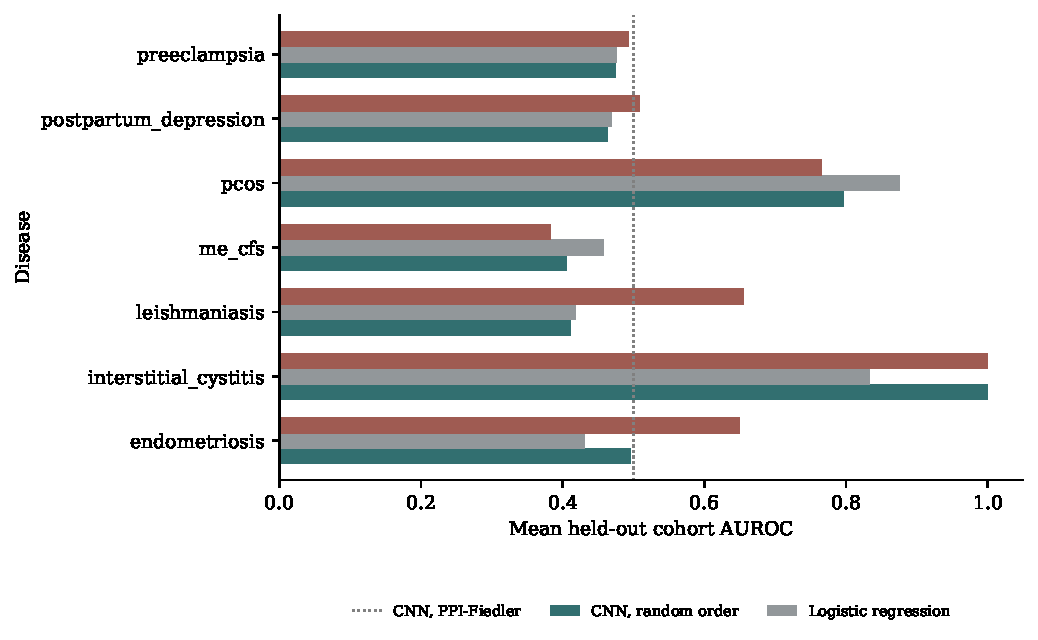
\includegraphics[width=.9\linewidth]{figures/cnn_crosscohort.pdf}\caption{Held-out cohorts by disease, calculated from \texttt{results/cnn\_crosscohort.csv} after deduplication. Mean AUROC is unweighted across validation cohorts within each disease; cohort sizes differ.}\end{figure}
\begin{figure}[ht]\centering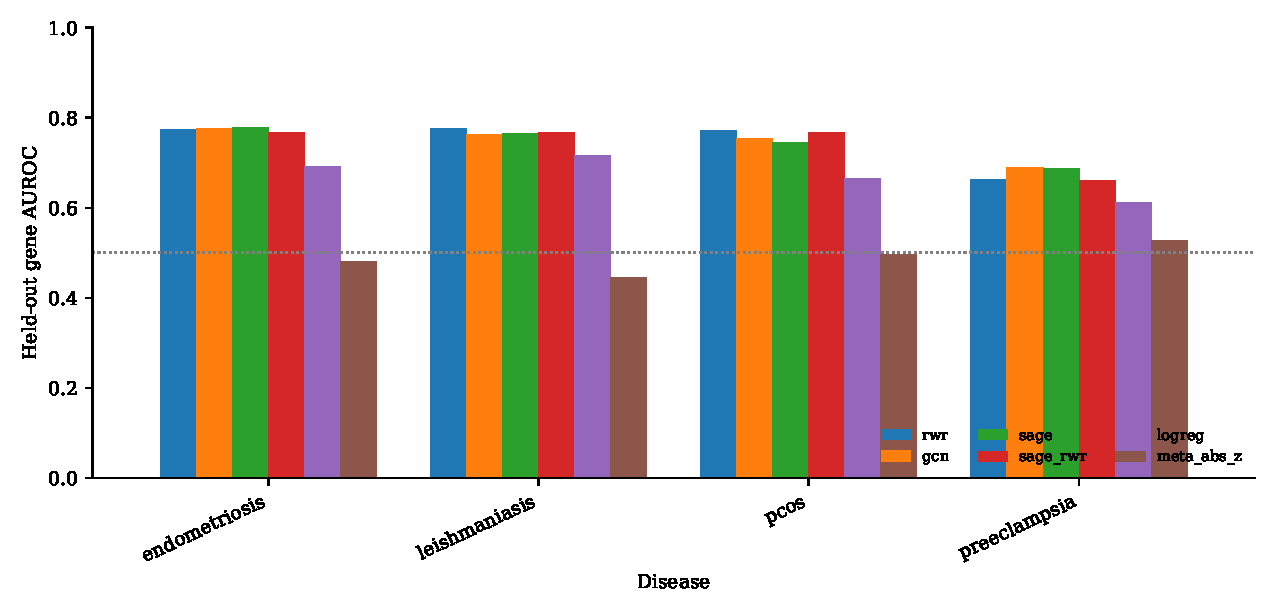
\includegraphics[width=.9\linewidth]{figures/gene_benchmark.pdf}\caption{Within-project gene-ranking benchmark. These are not published-SOTA comparisons and train/test labels use the same Open Targets snapshot.}\end{figure}
\clearpage\section{Prospective prediction attempts and failures}
P1, GNG2 down in preeclampsia, was registered before validation and failed (validation $p=0.24$). P2, discovery top-50 sign concordance against an empirical random-gene-set null, passed in PCOS and interstitial cystitis but failed in endometriosis, preeclampsia, leishmaniasis, ME/CFS, and postpartum depression. Interstitial cystitis validation has only seven samples. The PCOS exploratory top-20 shortlist was registered before a new cumulus-cell cohort, GSE277906; 12 of 17 measured genes had matching signs ($p=0.0717$, one-sided exact binomial, uncorrected). It does not meet the registered criterion and no q<0.05 gene was present in the deduplicated PCOS discovery meta-analysis.

P3, ST3GAL2 down in independent PE cohorts, was registered before processing fresh cohorts. The four-cohort random-effects standardized mean was $-0.1034$ with SE $0.3536$, one-sided $p=0.3850$ and $I^2=0.6874$. Restriction to three placenta-derived cohorts gave $-0.3739$, one-sided $p=0.0994$. Both fail; blood and one villus cohort point upward. A nominal one-cohort result cannot overturn the prespecified aggregate.
\begin{figure}[ht]\centering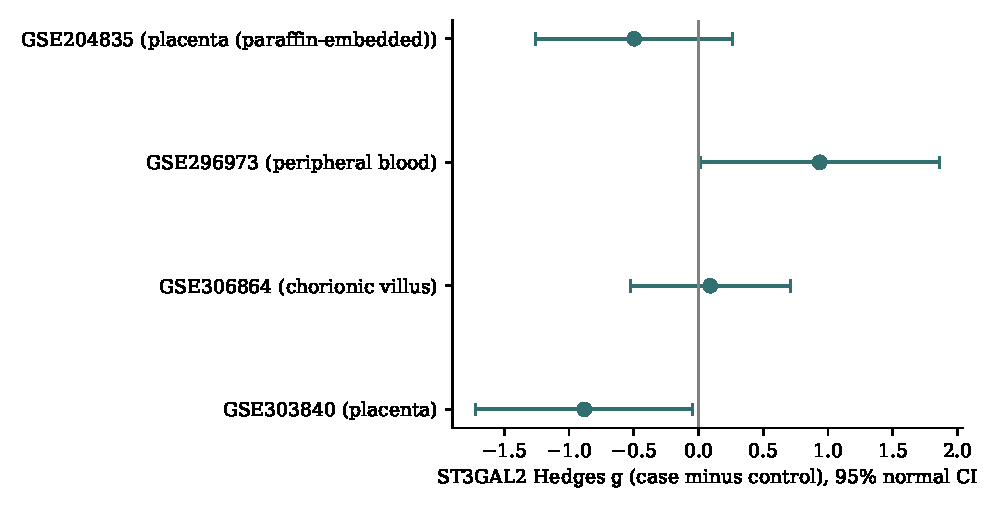
\includegraphics[width=.9\linewidth]{figures/P3_fresh_effects.pdf}\caption{Four fresh RNA-seq cohorts, direction and normal-reference intervals for ST3GAL2. Mixed tissues and one FPKM-normalized cohort are shown, not hidden.}\end{figure}
\subsection{Preeclampsia effect-estimator sensitivity}
The P3 ST3GAL2 decision used the registered DerSimonian--Laird pooled effect across all four fresh cohorts; it fails the one-sided down-regulation threshold ($p=0.3850$). As an estimator check, we recalculated from the same cohort effect sizes and variances with the independent \texttt{statsmodels} meta-analysis routine. Its DerSimonian--Laird result agrees numerically with the project implementation: $\hat\mu=-0.1034$, SE $0.3536$, and one-sided normal-reference $p=0.3850$. The iterative Paule--Mandel estimator returns $\hat\mu=-0.1016$, SE $0.3831$, $p=0.3955$. Leave-one-out iterative estimates also fail the $0.05$ down-direction threshold (one-sided $p$ range $0.0969$ to $0.6369$). Omitting the blood cohort yields the most favorable subset, $p=0.0969$; that is post-hoc and still negative. The independent-library check, generated from the same four cohort estimates, is in the PE P3 sensitivity CSV in the results folder. It does not add new cohorts. A small-$k$ random-effects model carries material uncertainty; choosing a different heterogeneity estimator cannot turn P3 into a discovery.

\subsection{All deduplicated signature replications}
The originally registered P2 statistic is sign agreement against 10,000 random gene sets. For a fixed set statistic $T$ and $B=10{,}000$ random sets, the empirical tail probability is
\begin{equation}\hat p_{\mathrm{emp}}=\frac{1+\sum_{b=1}^{B}\mathbf 1\{T_b\geq T_{\mathrm{obs}}\}}{B+1}.\end{equation}
 The next table lists all disease outcomes, including those with no usable validation cohort. The secondary T2 count combines matching sign with nominal within-validation $p<0.05$ and is also compared against the same gene-universe sampling logic. Repeating a signature test over many genes does not multiply the sample size: the unit of transport is the held-out cohort. A perfect concordance in seven interstitial cystitis validation samples is particularly fragile and requires a larger independent cohort. PCOS has a sign-set pass but no discovery gene at $q<0.05$, and later fresh-cohort tests show mixed transport. Preeclampsia's earlier apparent pass was invalidated by GSM overlap, as recorded rather than removed.
\begin{longtable}{lp{4.4cm}rrrrr}
\caption{Complete deduplicated top-50 discovery-signature replication results. T2 is the number of same-direction validation genes with nominal two-sided p below 0.05, assessed against random-gene sets; neither T2 nor the sign test is a clinical diagnostic metric.}\\
\hline Disease & GEO validation & Genes & Sign frac. & Emp. p & T2 & T2 p\\\hline\endfirsthead
\hline Disease & GEO validation & Genes & Sign frac. & Emp. p & T2 & T2 p\\\hline\endhead
chagas & none & -- & -- & -- & -- & --\\
endometriosis & GSE58178; GSE73622; GSE120103; GSE248593 & 47 & 0.64 & 0.1402 & 2 & 0.6903\\
fibromyalgia & none & -- & -- & -- & -- & --\\
interstitial\_cystitis & GSE57560 & 40 & 1.00 & 0.0001 & 22 & 0.0001\\
leishmaniasis & GSE125993 & 43 & 0.44 & 0.8496 & 4 & 0.5523\\
me\_cfs & GSE16059 & 50 & 0.30 & 0.9831 & 0 & 1.0000\\
pcos & GSE80432; GSE106724; GSE124226; GSE137684 & 50 & 0.72 & 0.0102 & 7 & 0.0078\\
postpartum\_depression & GSE290313-PP & 40 & 0.60 & 0.1259 & 2 & 0.3935\\
preeclampsia & GSE94643; GSE147776; GSE149440; GSE186819; GSE190639 & 49 & 0.53 & 0.2281 & 3 & 0.2662\\
\hline\end{longtable}

\section{Novelty and literature checks}
Open Targets absence is not biological novelty. Europe PMC returned two co-mentions for ST3GAL2 with preeclampsia at retrieval, whereas the earlier exact PubMed title/abstract query returned zero. The queries are not equivalent; the previous zero cannot support a novel-biology claim. Ensembl, UniProt, Reactome, MyGene.info, HGNC, GTEx reference, Human Protein Atlas, ClinVar and ChEMBL annotation responses are saved with exact URLs in \texttt{results/external/}. ChEMBL's ST3GAL2 target search returned a rat target but no human target among results; do not infer lack of druggability from this search alone. Human Protein Atlas links ST3GAL2 to ENSG00000157350 and reports protein-level evidence. ClinVar returns 105 gene-associated records for the exact ST3GAL2 gene query; this says nothing about preeclampsia association or a pathogenic allele in the condition. Neither source converts the falsified expression prediction into a clinical biomarker. An exact-trait GWAS Catalog lookup returned 145 preeclampsia association records and 18 author-reported gene-name mentions; neither ST3GAL2 nor GNG2 was among those names (\url{https://www.ebi.ac.uk/gwas/rest/api/efoTraits/MONDO_0005081/associations}). This limited author-reported-name search is not proof that either gene lacks genetic evidence, nor a test of placental expression. Published data serve as contextual sources, not a substitute for an independent held-out cohort.
\subsection{Physical-network context for the fixed panels}
The STRING physical-link graph underlying the GNN can check a narrower claim than pathway enrichment: whether a frozen sign panel is densely linked by recorded protein interactions. In the 50-gene IC discovery ranking, 35 symbols map to the score-400 physical graph and only one edge connects a pair; the largest induced component has two nodes. All 20 PCOS candidates map, but no pair has an edge at this threshold. A 1,000-draw random set from measured non-selected discovery genes gives means of 1.027 and 0.334 edges for IC and PCOS, respectively. These panels are not enriched for direct physical adjacency by this crude reference. The negative graph-context result does not deny co-regulation or shared inflammatory biology, which can occur without direct recorded physical links; nor does a degree-unmatched null license a pathway p-value. Missing STRING mappings (15 IC symbols) limit what the graph can say. The check uses a distinct graph-analysis library for connected components and saves its full result in \texttt{results/signature\_network\_context.json}. It provides an audit of a tempting mechanism claim rather than a new prediction target.


\subsection{Frozen six-gene preeclampsia panel: metadata failure and twin transport}
After viewing the old discovery and five-study validation summaries, a fixed screen selected six down-direction genes: FES, GPAT3, FURIN, GRAMD1A, ZNF467, and LPGAT1. Discovery required BH $q<0.05$ with at least eight cohorts, and old validation required concordant sign, nominal two-sided $p<0.01$ with at least three cohorts. Thus neither this selection nor its old validation is a new prospective discovery. The first fresh-cohort attempt, early chorionic-villus GSE295760, could not be tested reliably: GEO's series design describes 14 women (eight later PE, six controls), whereas the downloaded mRNA workbook and mRNA GSM metadata contain 19 columns/records (ten later PE, nine controls). Nineteen separate small-RNA records share participant tokens, but four tokens have opposite outcome labels between the two modalities: C1934, C1941, C3729, C4144. We excluded the whole cohort before computing any gene outcome. We did not count its 19 mRNA GSMs among used records. These are public metadata contradictions, not evidence of fraud or a biological finding (\url{https://www.ncbi.nlm.nih.gov/geo/query/acc.cgi?acc=GSE295760}).

The independently registered transport attempt P10 used GSE272342 villous twin placentas, a different population and gestational context from the intended early-CVS prediction (\url{https://www.ncbi.nlm.nih.gov/geo/query/acc.cgi?acc=GSE272342}). Its 32 twin GSM counts belong to 16 pregnancies, not 32 independent observations. We applied log$_2$(counts per million$+1$) to each sample, averaged siblings within a pregnancy, then compared seven PE pregnancies with nine normotensive pregnancies. Thirteen singleton PE samples were excluded, three of which are resequencings of persons in GSE203507; no singleton controls were present. Pregnancy-level Hedges effects (uncorrected Welch $p$ in parentheses) were FES $-1.524$ (.0091), GPAT3 $+0.488$ (.322), FURIN $+0.062$ (.894), GRAMD1A $-1.189$ (.0395), ZNF467 $-0.844$ (.0775), and LPGAT1 $-0.199$ (.6645). Four of six signs agreed; two reversed. The six measured effects and their uncertainty are tabulated below. Even nominal FES evidence does not pass a six-gene Bonferroni threshold of $.05/6=.00833$. The registered empirical matched-direction null was inoperable: exactly six genes met the earlier eligibility filter, all already in the selected panel, so no disjoint six-gene sets could be drawn. We did not choose a new null after seeing the outcomes. Thus neither P9 nor P10 provides the independent, corrected replication required for a biomarker claim. \begin{longtable}{lrrl}
\caption{P10 twin-placenta results for the six frozen down-direction genes. Each Hedges $g$ is computed on 16 pregnancy means (7 PE, 9 controls), not 32 sibling samples. Welch $p$ is uncorrected and the panel fails: two genes reverse. The post-result adjusted FES test does not change this prespecified panel conclusion. Source: results/pe\_twin\_p10.csv.}\\
\hline Gene & Hedges $g$ & Welch $p$ & Observed\\\hline\endfirsthead
\hline Gene & Hedges $g$ & Welch $p$ & Observed\\\hline\endhead
FES & -1.524 & 0.0091 & down\\
GPAT3 & +0.488 & 0.3218 & up\\
FURIN & +0.062 & 0.8944 & up\\
GRAMD1A & -1.189 & 0.0395 & down\\
ZNF467 & -0.844 & 0.0775 & down\\
LPGAT1 & -0.199 & 0.6645 & down\\
\hline\end{longtable}

The exact sample map, effects, and exclusion are retained in the repository. A later, explicitly post-outcome sensitivity found that FES remains down in all sixteen leave-one-pregnancy-out fits and has max-absolute-Welch-$t$ permutation familywise $p=0.0342$ across the six genes under all 11,440 label assignments. A separate descriptive regression including gestational age at delivery gave FES case coefficient $-0.344$ log$_2$ CPM and nominal $p=0.00848$; mean delivery ages were 33.20 and 33.11 weeks for PE and controls. These analyses were devised after seeing cohort effects, and delivery age may be affected by PE. They neither replace the infeasible registered matched-gene null nor overcome the failed six-gene panel, twin case-mix, or lack of a matching independent cohort.

\subsection{P11 early plasma cfRNA transport: another negative}
We next fixed the same six directions before downloading GSE192902's count matrices, using the first $\leq12$-week plasma cell-free RNA draw per mother in each of the three named internal cohorts (\url{https://www.ncbi.nlm.nih.gov/geo/query/acc.cgi?acc=GSE192902}). All 404 GEO sample titles mapped to the post-QC count columns, and no maternal ID crossed cohorts. We retained Discovery 13 PE and 36 controls, Validation 1 three PE and 19 controls, and Validation 2 sixteen PE and 40 controls, totaling 127 first prenatal draws. The gene GPAT3 was absent in all count matrices; five of six panel genes could be evaluated. The frozen downward direction agreed for just 2/5, 1/5, and 3/5 genes in the three cohorts, far below the registered 5/5 criterion. FES standardized effects were $+0.036$ ($p=0.912$), $-0.402$ ($p=0.680$), and $-0.361$ ($p=0.215$), respectively. No gene reached the corrected threshold in two internal cohorts. \begin{longtable}{lp{3.0cm}p{3.0cm}p{3.0cm}}
\caption{P11 first-$\leq12$-week plasma cfRNA transport effects. Each cell is Hedges $g$ (uncorrected two-sided Welch $p$), PE minus controls; negative is the frozen predicted direction. Discovery: 13/36 PE/control mothers; Validation 1: 3/19; Validation 2: 16/40. GPAT3 is not measurable. These internal cohorts come from one GSE, and none passes the five-of-five down-sign rule. Source: results/pe\_cfrna\_p11.csv.}\\
\hline Gene & Discovery & Validation 1 & Validation 2\\\hline\endfirsthead
\hline Gene & Discovery & Validation 1 & Validation 2\\\hline\endhead
FES & +0.04 (0.912) & -0.40 (0.680) & -0.36 (0.215)\\
GPAT3 & not measured & not measured & not measured\\
FURIN & +0.44 (0.224) & +0.86 (0.082) & +0.26 (0.377)\\
GRAMD1A & -0.19 (0.663) & +1.22 (0.133) & +0.00 (0.986)\\
ZNF467 & +0.26 (0.379) & +0.31 (0.763) & -0.22 (0.505)\\
LPGAT1 & -0.10 (0.802) & +0.42 (0.117) & -0.25 (0.390)\\
\hline\end{longtable}

The expression modality is circulating RNA, not placental tissue; this failed transport cannot refute a tissue-specific placental FES effect, but it does block a claim of general early blood-based predictive portability. These 127 sample IDs are nested in one GSE, not independent studies. The full sample mappings and every measured effect remain in \texttt{results/pe\_cfrna\_p11.csv} and its companion ledgers.


\subsection{P12-P13 placental challenges of a fixed six-gene panel}
We next checked the same frozen six DOWN directions in three placental GEO deposits, with the decisions registered before each deposit's expression matrix was opened. They are not new discoveries: the panel was chosen using old discovery and validation outcomes and examined in P10 and P11 before these studies. A fresh study-level outcome cannot restore the original prospective status. The studies also differ in disease severity, fetal-growth-restriction status, gestational timing and expression processing. The statistical unit is one woman in each of these three deposits, rather than the twin placenta in P10 or repeated draw in P11.

In GSE190971 we used only the thirteen placenta mRNA samples, seven PE and six controls, rather than the 10K and 150K extracellular-vesicle arms, which share participant identifiers with the placenta samples (\url{https://www.ncbi.nlm.nih.gov/geo/query/acc.cgi?acc=GSE190971}). All thirteen raw-count columns mapped to unique GEO titles and GSMs and the related assay arms had consistent per-person phenotype labels. On log$_2$(CPM+1), FES was down with Hedges $g=-2.800$ and uncorrected two-sided Welch $p=0.000372$, below the six-gene Bonferroni threshold $0.00833$. GPAT3 was up, $g=+0.161$, $p=0.757$; the other four genes were down. The registered all-six-down panel criterion therefore fails at five of six, despite the strong FES component. Recounting the repeated EV arms as independent people would be false replication. All six gene effects and per-GSM count mappings are in \texttt{results/pe\_plac\_p12*}.

P13 specified a two-study test of the same six signs. GSE186257 provided a deposited filtered, DESeq2-normalized matrix, not raw counts, and all 44 columns mapped exactly to GEO titles and GSMs (26 severe PE, 18 nonhypertensive controls; \url{https://www.ncbi.nlm.nih.gov/geo/query/acc.cgi?acc=GSE186257}). After log$_2$(normalized value+1), all six effects pointed down. FURIN $g=-1.033$, $p=0.000559$ and ZNF467 $g=-0.965$, $p=0.00209$ passed the local six-gene threshold; FES was down $g=-0.665$, nominal $p=0.0209$ but not corrected. This single-study success does not meet the P13 two-study rule.

GSE114691 sampled placentas at birth. Its 21 control and 20 PE-only count columns mapped one-to-one through GEO's sample-description tokens to unique GSMs; the separate 18 IUGR-only and 20 PE+IUGR samples were excluded from the primary test (\url{https://www.ncbi.nlm.nih.gov/geo/query/acc.cgi?acc=GSE114691}). The release uses \texttt{ENST} transcript IDs, unlike the other gene-level matrices. A documented Ensembl transcript membership lookup found 17 FES, seven GPAT3, three FURIN, fourteen GRAMD1A, two ZNF467 and four LPGAT1 transcript IDs in the historical file. Summing each gene's matched transcript counts and applying log$_2$(CPM+1) gave FES $g=-1.537$, Welch $p=0.000014$, but FURIN reversed ($g=+0.423$, $p=0.172$). Five of six directions agreed, so the registered two-study panel criterion \emph{fails}. Current Ensembl transcript membership may omit historical hg19 isoforms; this analysis is a bounded gene-extraction sensitivity, not an exhaustive original annotation reprocessing. The exact selected transcript IDs, source checksums, column-to-GSM mapping, and six effects are recorded in \texttt{results/pe\_plac\_p13*} and \texttt{results/external/p13\_ensembl\_transcript\_map.json}. The RCSB Protein Data Bank identifies resolved human FES kinase structures, including 8XKP (2.05~\AA) and 3BKB (1.78~\AA), and confirms the protein is not a purely in-silico gene label (\url{https://www.rcsb.org/structure/8XKP}; \url{https://www.rcsb.org/structure/3BKB}). Crystal structures establish molecular context only: they do not show PE association, placental mechanism, treatment efficacy, or safety in pregnancy. Separately, BioGRID records 40 interactors and 53 curated interactions for the human FES record, with BCR and HSH2D example interaction pages using affinity capture and other experimental assays (\url{https://thebiogrid.org/108533/summary/homo-sapiens/fes.html}; \url{https://thebiogrid.org/interaction/317111}). Interactions from assorted tissues and studies do not identify a PE causal pathway or support clinical use. GlyGen independently curates ten FES phosphorylation-site entries, including two source-specific records at Tyr713 for P07332-1 (\url{https://glygen.org/protein/P07332-1}; API \url{https://api.glygen.org/protein/detail/P07332-1}). These are site entries rather than ten unique residues or placental phosphoproteomics; RNA abundance cannot establish kinase activity. The returned tissue and disease expression subsets lack placenta and PE entries, but absence in these limited lists is not evidence of biological absence. The separate iPTMnet P07332 entry lists FES as a phosphorylation enzyme for BCR Y177 and PECAM1 Y690 (\url{https://research.bioinformatics.udel.edu/iptmnet/entry/P07332/}). It aggregates overlapping literature and databases, not a separate placenta-specific kinase experiment; these example substrates do not establish a PE pathway. This repeated down FES effect in nonexchangeable at-birth placental cohorts is a falsifiable descriptive signal, but because FES was selected after the earlier panels, has tissue and case-mix confounding, and lacks an untouched prospectively sampled pregnancy cohort, it does not yet satisfy a novel biomarker claim. The three new GSEs contribute 98 used GSM accession records, not 98 new studies. An additional source-metadata check sharpens the confounding limit: in GSE190971, all six normal-placenta controls are recorded without IUGR and delivered from 38 to 41+2 weeks, while six of seven PE records are marked IUGR and their legible delivery ages range from 27+1 to 35+5 weeks. The seventh PE record has malformed or absent fields at the expected positions, so it is not assigned an IUGR or delivery-age value. In GSE186257, small-for-gestational-age status occurs in 25/26 severe PE versus 8/18 controls. Thus the repeated FES placenta effect cannot be separated from growth restriction, gestational timing or tissue composition by these comparisons. These imbalances are from the GEO sample metadata, not fitted adjustment results. An explicitly post-outcome within-study SGA stratum check in GSE186257 retains 25 severe PE and 8 controls: FES is still down ($g=-0.629$) but its uncorrected Welch $p=0.0718$. There is just one non-SGA PE, so a non-SGA contrast cannot estimate a reliable variance. Male-only (12/12) FES has $g=-0.857$, $p=0.0440$; female-only (14/6) has $g=-0.530$, $p=0.227$. These descriptive strata are small, were selected after viewing the group imbalance, and cannot causally adjust for an SGA label possibly downstream of PE. A further post-selection descriptive four-study random-effects combination of the already inspected FES placental effects gives $g=-1.458$, between-study $\tau^2=0.414$ and raw $I^2=0.637$. A normal-reference 95\% interval $[-2.250,-0.666]$ excludes zero, but a rough 95\% prediction interval $[-2.947,+0.031]$ crosses zero. With only four discordant studies, Hartung--Knapp $t$ reference yields $p=0.0366$; leave-one-study-out $p$ ranges from $0.0339$ to $0.1303$, and the non-twin three-study sensitivity yields $p=0.1223$. These calculations were performed after FES was selected and observed in all cohorts, so none is an independent confirmation or a PE-specific effect. Exact input rows and output are in \texttt{results/pe\_fes\_placenta\_meta\_cohorts.csv} and its exploratory JSON. Full six-gene subgroup effects are in \texttt{results/pe\_p13\_sga\_sensitivity.csv}.

\subsection{P14 re-mapped hypertensive-disorder deposit: a reuse-risk challenge}
A later GEO deposit, GSE303463, supplies raw placental count columns for 168 GSMs across two sequencing platforms (\url{https://www.ncbi.nlm.nih.gov/geo/query/acc.cgi?acc=GSE303463}). Its own study design says previously derived GSE186257, GSE234729, and PRJNA1027377 material was re-mapped alongside newly derived material. Because GSE186257 was already used for P13, distinct identifiers in the later deposit are not evidence of independent participants. We recorded an exploratory analysis plan before opening this deposit's FES count row, but FES had already been selected and tested in earlier cohorts. P14 cannot be a prospective discovery or independent replication. These 168 new GSM identifiers are omitted from the used-accession tally pending patient-level source mapping.

All 168 raw-count title columns mapped one-to-one to the GEO series-matrix GSM identifiers. We normalized each sample by its mapped-count library total, computed log$_2$(CPM$+1$), and compared disease exactly PE with exactly Normal, excluding superimposed PE and chronic/gestational hypertension. All 22 PE cases were on the GPL34281 platform; the pooled 22 PE/68 Normal contrast mixes platform with disease, despite its FES Hedges $g=-0.991$ and nominal Welch $p=6.82\times10^{-6}$. Restricting to GPL34281 gives 22 PE/60 Normal, $g=-0.944$, $p=0.000320$. The age-overlap 34--39-week subset gives 13/41, $g=-1.130$, $p=0.000700$; these are delivery, not prediagnostic, ages. Median delivery week is 35 in PE versus 39 in Normal. Placental maternal vascular malperfusion (MVM) is recorded in 13/22 PE and 4/68 Normal. Within GPL34281, non-MVM gives 9/56, $g=-1.211$, $p=0.0146$, while MVM gives 13/4, $g=-0.434$, $p=0.582$. A descriptive same-platform OLS conditioned on gestational week and MVM gives a PE coefficient of $-0.380$ log$_2$(CPM$+1$), nominal $p=0.00728$, but conditioning on delivery pathology or week can introduce mediation and selection bias. None of these post-selected, potentially reused contrasts establishes specificity to PE, diagnosis before delivery, clinical utility, or a new discovery. The matrix SHA-256, exact per-GSM map and every group count are in \texttt{results/pe\_p14\_*}; the analysis script is \texttt{scripts/pe\_p14\_hdp\_reuse\_diagnostic.py}. The source authors' paper (DOI \url{https://doi.org/10.1161/atvbaha.125.323457}) also frames its cohort as previously and newly obtained RNA-seq material.

\section{Limitations and next work}
Sample labels may be wrong where GEO metadata are incomplete; all included labels require audit. Cross-platform effect sizes standardize units but do not remove tissue, gestational-age, or case-definition confounding. Four PE cohorts differ in tissue, and a single PCOS cumulus cohort is insufficient for discovery. The exploratory PCOS gene signs in GSE304677 (17/18 measured) are not a registered confirmatory discovery; a post-hoc, direction-matched null gives $p=0.0021$, while GSE277906 does not pass the naive $p=0.05$ threshold. After registration, GSE155489 showed 16/17 signs and direction-matched $p=0.0139$, but PBMC GSE262735 had 11/17 signs ($p=0.1951$), pooled-library granulosa GSE193123 had 12/18 ($p=0.1795$), and a new 9-case/9-control follicular-granulosa cohort GSE293353 had 16/19 ($p=0.5884$ under its direction-matched null). These are mixed, not consistent validation. GSE173160 supplied 177,889 transcript IDs with no direct HGNC symbol matches and was excluded from this test by the registered mapping rule. A mostly upward selected gene set against an overall upward cohort shift makes a half-probability binomial null anti-conservative. One study can have multiple data depositions: unique accessions do not equal independent studies. We will count both levels and keep the accession-to-study mapping explicit. Only a comparison on matching published benchmark inputs and splits or an untouched, corrected, named discovery can satisfy the discovery gate. No clinical diagnostic inference is warranted.

\section{Full cohort-level results and endpoint boundaries}
\subsection{Discovery availability and fragility}
Nine disease labels had a case/control expression discovery analysis after filtering; the tenth requested label did not have a usable human comparison in the searched records. The discovery-summary table records an especially uneven disease footprint. One-series Chagas, fibromyalgia and postpartum depression estimates cannot identify a between-study variance. A large number of significant genes from one setting does not by itself imply transport across tissues, collection protocols or patient populations. Preeclampsia draws on sixteen discovery series but spans blood and placental compartments; the total count alone is not a measure of homogeneity.

\subsection{Full fresh-cohort disposition}
The table below is generated from the exact committed per-cohort source ledger. The nine listed supplementary expression matrices are not exchangeable: the placenta, blood, villus, cumulus and ovarian granulosa materials each answer different biological questions. Each supplementary-matrix study is displayed once even when several registered hypotheses examined it; the separate GSE28242 series-matrix P7 and GSE293353 count-matrix P8 are analyzed later and are not silently part of this nine-row table. Case and control totals are library-level observations as in the GEO sample matrix; GSE193123 pooled two individuals into each library, so six libraries cannot be treated as twelve independent people. GEO's metadata and supplementary matrices can be opened from the accession and exact links recorded in the source CSV.
\begin{longtable}{llrrrp{4.5cm}l}
\caption{Fresh RNA-seq cohorts and sample-library counts. Source URLs and complete metadata are in results/fresh\_rnaseq\_summary.csv. These series were not all used for the same hypothesis; an included row is not an independent replication of every candidate.}\label{tab:fresh}\\
\hline GEO & Disease & Cases & Controls & Genes & Tissue & Unit\\\hline\endfirsthead
\hline GEO & Disease & Cases & Controls & Genes & Tissue & Unit\\\hline\endhead
GSE155489 & pcos & 4 & 4 & 22064 & cumulus granulosa cells & counts\\
GSE262735 & pcos & 9 & 9 & 16655 & PBMC monocytes & counts\\
GSE277906 & pcos & 23 & 17 & 13716 & cumulus cells & counts\\
GSE304677 & pcos & 5 & 5 & 17439 & ovarian granulosa cells & counts\\
GSE204835 & preeclampsia & 16 & 12 & 16247 & placenta (paraffin-embedded) & counts\\
GSE296973 & preeclampsia & 10 & 10 & 33326 & peripheral blood & FPKM\\
GSE303840 & preeclampsia & 12 & 12 & 16264 & placenta & counts\\
GSE306864 & preeclampsia & 13 & 45 & 15118 & chorionic villus & counts\\
GSE193123 & pcos & 3 & 3 & 16137 & ovarian granulosa cells pooled libraries & counts\\
\hline\end{longtable}


\subsection{All graph-ranking comparisons}
Table~\ref{tab:gene} expands the compact plot into every disease and tested method. The gene-recovery labels are defined from the same ontology/evidence collection used to construct the project; although the held-out folds avoid a gene's training label, they are not future clinical outcomes. Thus fold AUROC can evaluate the internal ranking task only. For postpartum depression, the mean GCN AUROC is 0.695 against 0.803 for random walk with restart; a strong generic graph baseline matters more than comparing against an unrelated published endpoint. For other diseases a small apparent GCN advantage over RWR is not a published benchmark break and should be evaluated under multiple seeds and an external label freeze before it is promoted. Rare positive labels mean AUPRC is also reported: AUROC alone hides precision limitations in a large candidate universe.
\begin{longtable}{llrrr}
\caption{Mean within-project held-out gene-recovery fold metrics. Positive labels derive from the selected Open Targets snapshot, not a temporally independent clinical endpoint. Methods and folds are given in the repository CSVs.}\label{tab:gene}\\
\hline Disease & Model & Folds & AUROC & AUPRC\\\hline\endfirsthead
\hline Disease & Model & Folds & AUROC & AUPRC\\\hline\endhead
chagas & gcn & 10 & 0.761 & 0.073\\
chagas & logreg & 10 & 0.668 & 0.039\\
chagas & meta\_abs\_z & 10 & 0.509 & 0.024\\
chagas & mlp & 10 & 0.653 & 0.038\\
chagas & rwr & 10 & 0.774 & 0.071\\
chagas & sage & 10 & 0.733 & 0.064\\
chagas & sage\_rwr & 10 & 0.758 & 0.069\\
endometriosis & gcn & 10 & 0.777 & 0.293\\
endometriosis & logreg & 10 & 0.692 & 0.177\\
endometriosis & meta\_abs\_z & 10 & 0.481 & 0.089\\
endometriosis & mlp & 10 & 0.698 & 0.181\\
endometriosis & rwr & 10 & 0.774 & 0.321\\
endometriosis & sage & 10 & 0.779 & 0.295\\
endometriosis & sage\_rwr & 10 & 0.768 & 0.303\\
fibromyalgia & gcn & 10 & 0.790 & 0.069\\
fibromyalgia & logreg & 10 & 0.708 & 0.041\\
fibromyalgia & meta\_abs\_z & 10 & 0.530 & 0.028\\
fibromyalgia & mlp & 10 & 0.699 & 0.032\\
fibromyalgia & rwr & 10 & 0.850 & 0.126\\
fibromyalgia & sage & 10 & 0.788 & 0.056\\
fibromyalgia & sage\_rwr & 10 & 0.840 & 0.110\\
interstitial\_cystitis & gcn & 10 & 0.720 & 0.048\\
interstitial\_cystitis & logreg & 10 & 0.624 & 0.024\\
interstitial\_cystitis & meta\_abs\_z & 10 & 0.485 & 0.015\\
interstitial\_cystitis & mlp & 10 & 0.629 & 0.031\\
interstitial\_cystitis & rwr & 10 & 0.710 & 0.061\\
interstitial\_cystitis & sage & 10 & 0.678 & 0.051\\
interstitial\_cystitis & sage\_rwr & 10 & 0.708 & 0.057\\
leishmaniasis & gcn & 10 & 0.763 & 0.225\\
leishmaniasis & logreg & 10 & 0.717 & 0.133\\
leishmaniasis & meta\_abs\_z & 10 & 0.445 & 0.040\\
leishmaniasis & mlp & 10 & 0.718 & 0.143\\
leishmaniasis & rwr & 10 & 0.777 & 0.179\\
leishmaniasis & sage & 10 & 0.765 & 0.213\\
leishmaniasis & sage\_rwr & 10 & 0.768 & 0.156\\
me\_cfs & gcn & 10 & 0.765 & 0.126\\
me\_cfs & logreg & 10 & 0.690 & 0.054\\
me\_cfs & meta\_abs\_z & 10 & 0.485 & 0.029\\
me\_cfs & mlp & 10 & 0.689 & 0.045\\
me\_cfs & rwr & 10 & 0.806 & 0.142\\
me\_cfs & sage & 10 & 0.766 & 0.115\\
me\_cfs & sage\_rwr & 10 & 0.793 & 0.128\\
pcos & gcn & 10 & 0.753 & 0.306\\
pcos & logreg & 10 & 0.665 & 0.181\\
pcos & meta\_abs\_z & 10 & 0.495 & 0.098\\
pcos & mlp & 10 & 0.670 & 0.185\\
pcos & rwr & 10 & 0.772 & 0.325\\
pcos & sage & 10 & 0.745 & 0.304\\
pcos & sage\_rwr & 10 & 0.767 & 0.307\\
postpartum\_depression & gcn & 10 & 0.695 & 0.006\\
postpartum\_depression & logreg & 10 & 0.582 & 0.012\\
postpartum\_depression & meta\_abs\_z & 10 & 0.561 & 0.003\\
postpartum\_depression & mlp & 10 & 0.531 & 0.004\\
postpartum\_depression & rwr & 10 & 0.803 & 0.028\\
postpartum\_depression & sage & 10 & 0.642 & 0.005\\
postpartum\_depression & sage\_rwr & 10 & 0.775 & 0.025\\
preeclampsia & gcn & 10 & 0.691 & 0.279\\
preeclampsia & logreg & 10 & 0.612 & 0.189\\
preeclampsia & meta\_abs\_z & 10 & 0.527 & 0.155\\
preeclampsia & mlp & 10 & 0.618 & 0.195\\
preeclampsia & rwr & 10 & 0.663 & 0.260\\
preeclampsia & sage & 10 & 0.687 & 0.268\\
preeclampsia & sage\_rwr & 10 & 0.660 & 0.253\\
\hline\end{longtable}


\subsection{Paired graph-baseline comparisons within the project}
Each gene-ranking method shares the same Open Targets label folds, so its comparison with random walk with restart (RWR) is naturally paired within a disease. The ten available folds are two random repetitions of five-fold gene cross-validation on one graph, not ten independent validation studies. On the internal label-recovery endpoint, preeclampsia GCN exceeds RWR in all ten AUROC folds and nine of ten AUPRC folds: mean AUROC 0.691 versus 0.663, mean AUPRC 0.279 versus 0.260. This modest advantage is not a published-SOTA benchmark break, because it is within-project with one label snapshot and a baseline tuned under its own implementation. Postpartum depression points in the opposite direction (GCN AUROC 0.695 versus RWR 0.803; AUPRC 0.0056 versus 0.0275). PCOS also favors RWR in all ten AUROC folds (0.772 versus 0.753), and interstitial cystitis has a GCN AUROC gain of only 0.0094 while RWR has better AUPRC (0.0608 versus 0.0482). The full paired comparison across nine diseases and both metrics is \texttt{results/gene\_fold\_uncertainty.csv}; exploratory fold-level signed-rank p-values cannot be interpreted as external replication because folds reuse genes, edges and disease label sources. The AUPRC reversals warn against picking only the most flattering ranking metric.

\subsection{All held-out patient-classifier cohorts}
The cohort-wise CNN table discloses every tested holdout rather than selected wins. Across 17 holdouts, the mean CNN AUROC is 0.578 and the logistic baseline is 0.628 (unweighted over cohorts). The CNN with randomized gene order is an ablation; an ordering effect, even when present in one cohort, does not confer clinical usefulness. Results vary across cohorts because sample sizes, assay technologies, tissue and phenotype definitions vary. The classifier learns from a training cohort but is evaluated on a different GEO deposit; this guards against within-cohort leakage but not against every form of selection bias or shared participant identifiers. The accession split and GSM overlap checks are therefore part of the analysis, not clerical cleanup.
\begin{longtable}{llrrrrr}
\caption{Every held-out validation cohort, including poor CNN results. Test sizes are sample counts, not independent cohorts. No row is a published-benchmark comparison.}\label{tab:cnn}\\
\hline Disease & GEO & Train n & Test n & CNN & Random-order CNN & Logistic\\\hline\endfirsthead
\hline Disease & GEO & Train n & Test n & CNN & Random-order CNN & Logistic\\\hline\endhead
endometriosis & GSE58178 & 313 & 12 & 0.528 & 0.472 & 0.833\\
endometriosis & GSE73622 & 313 & 50 & 0.593 & 0.521 & 0.420\\
endometriosis & GSE120103 & 313 & 36 & 0.583 & 0.534 & 0.759\\
endometriosis & GSE248593 & 313 & 12 & 0.278 & 0.194 & 0.583\\
interstitial\_cystitis & GSE57560 & 30 & 7 & 1.000 & 0.833 & 1.000\\
leishmaniasis & GSE125993 & 65 & 45 & 0.412 & 0.418 & 0.655\\
me\_cfs & GSE16059 & 30 & 76 & 0.405 & 0.457 & 0.383\\
pcos & GSE80432 & 103 & 12 & 0.906 & 0.844 & 0.750\\
pcos & GSE106724 & 103 & 8 & 0.938 & 1.000 & 0.938\\
pcos & GSE124226 & 103 & 8 & 0.625 & 0.812 & 0.500\\
pcos & GSE137684 & 103 & 12 & 0.719 & 0.844 & 0.875\\
postpartum\_depression & GSE290313-PP & 48 & 184 & 0.463 & 0.469 & 0.508\\
preeclampsia & GSE94643 & 672 & 16 & 0.422 & 0.375 & 0.797\\
preeclampsia & GSE147776 & 672 & 21 & 0.346 & 0.385 & 0.269\\
preeclampsia & GSE149440 & 672 & 380 & 0.442 & 0.558 & 0.507\\
preeclampsia & GSE186819 & 672 & 25 & 0.628 & 0.500 & 0.481\\
preeclampsia & GSE190639 & 672 & 19 & 0.538 & 0.564 & 0.410\\
\hline\end{longtable}


\subsection{Cohort-level uncertainty for the CNN comparison}
The difference in AUROC for each of the 17 cohort holdouts is paired: the CNN and logistic model face the same held-out sample set. The unweighted mean difference is $-0.0496$ (CNN minus logistic), compared with $-0.0481$ when weighted by validation sample count. Of 17 holdouts, the CNN wins seven, loses eight, and ties two; a two-sided sign test on the 15 non-ties yields $p=1.00$, and a paired Wilcoxon test yields $p=0.293$. A seed-fixed 10,000-resample bootstrap over the 17 cohort differences returns a percentile interval $[-0.133,0.030]$. It spans zero, so the point estimate does not establish statistical superiority of logistic regression in a population. Excluding the seven-sample interstitial-cystitis validation cohort leaves an unweighted mean difference of $-0.0527$, not a reversal. These checks are reproducible from \texttt{results/cnn\_uncertainty.json}; resampling selected GEO cohorts as if exchangeable ignores repeated disease families and tissue heterogeneity, so the bootstrap is descriptive rather than a generalizable inferential interval. The test sample count weighting also allows one large cohort to dominate. A controlled new prospective cohort, or an external matched-task benchmark, would be needed for a stronger comparison.

\subsection{PCOS follow-up with a null matched to selection}
The original exploratory 20-gene set was chosen mostly from positive discovery effects, which makes a symmetric coin-flip null misleading whenever a validation cohort has an overall positive drift. We therefore drew 10,000 gene sets from the intersection of discovery and validation genes, excluding the target set, preserving the numbers with positive and negative discovery effects and a minimum four-discovery-cohort availability. The empirical $p$ estimates in Table~\ref{tab:pcos} measure how unusually many signs agree under this conditional gene universe. They are not a diagnosis-level sensitivity or specificity estimate. The positive GSE155489 result is a small cumulus-cell cohort; the other tissue and pooled-library tests were negative. A second confirmatory matched-tissue cohort was unavailable under the registered ID-mapping rule. Any claim that this fixed sign panel is established or that any one of its genes is novel would be premature.
\begin{longtable}{lrrrrp{3cm}}
\caption{Registered PCOS top-20 sign-set tests with a discovery-direction- and coverage-matched empirical null. Signs are the count agreeing among measured candidates, not gene-level significance. GSE193123 has three pooled case and three pooled control libraries.}\label{tab:pcos}\\
\hline GEO & Signs & Matched & Null mean & Empirical p & Cell type\\\hline\endfirsthead
\hline GEO & Signs & Matched & Null mean & Empirical p & Cell type\\\hline\endhead
GSE155489 & 16/17 & 16+/1- & 11.73 & 0.0139 & cumulus\\
GSE262735 & 11/17 & 16+/1- & 8.68 & 0.1951 & PBMC monocytes\\
GSE193123 & 12/18 & 17+/1- & 9.54 & 0.1795 & granulosa, pooled\\
\hline\end{longtable}



\begin{figure}[ht]\centering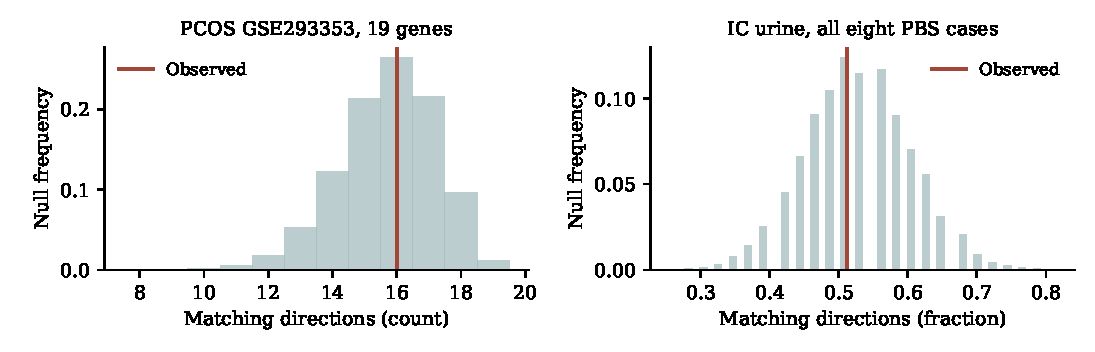
\includegraphics[width=.96\linewidth]{figures/matched_null_failures.pdf}\caption{Selection-matched null distributions for the 19 measurable PCOS genes in GSE293353 and the 43 measurable IC genes in the all-PBS urine comparison. The red line is observed agreement. A high raw sign fraction can be ordinary when the selected directions and cohort-wide shift make matching likely. Null draws and seeds are in committed CSV files; the panels summarize failed registered primary tests, not diagnostic performance.}\end{figure}
\section{A second matched-tissue PCOS null result}
Before inspecting GSE293353 expression, we froze the original twenty discovery-ranked PCOS signs and the same 10,000-set direction- and discovery-coverage-matched null. The study deposited bulk RNA-seq of follicular granulosa cells from nine patients with PCOS and nine controls (\url{https://www.ncbi.nlm.nih.gov/geo/query/acc.cgi?acc=GSE293353}). Its clinical sample-information file, GEO titles and count columns form an exact one-to-one name-to-GSM mapping; none of those 18 GSMs overlaps previously processed PCOS samples. The matrix's Ensembl IDs map through the local HGNC set; three IDs with competing approved symbols are excluded instead of assigned arbitrarily. We apply a per-library CPM transform and keep genes above 1 CPM in at least 20\% of libraries before log2(CPM+1) and a case-control standardized mean contrast. Source and SHA-256 checksums, complete sample mapping, and each selected gene's effect are retained in \texttt{results/pcos\_p8*}.

Nineteen of the frozen twenty genes remain measurable. Sixteen directions agree, which alone seems promising; the matched null expects 15.725 agreements, and its empirical $p=0.5884$ fails the registered $0.025$ threshold. This is a particularly clear example of why a naive half-probability sign test is misleading for a set with eighteen positive and one negative discovery signs in a cohort with strong global directional drift. GSE293353 includes authors' integrative analyses of other public PCOS data; absent duplicate GSMs prevents direct sample leakage in this test but does not make its literature claims or methods independent of every other GEO study. This result does not undo the small GSE155489 positive; it limits its generality. After seeing the P8 outcomes, an exploratory mean of within-cohort standardized expression signed by the frozen panel yielded AUROC 0.815 and AUPRC 0.857 in these same eighteen samples. A 1,000-draw random-sign baseline had AUROC mean 0.504 and empirical $p=0.060$. Neither metric was registered as P8's primary outcome, and normalizing on all P8 samples uses the evaluation distribution itself. This is not a clinical score or published head-to-head benchmark. A patient-level assay requires predeclared gene-level measurement, a locked classifier threshold and external clinical validation, not a sign fraction alone.

\section{Interstitial cystitis: a registered cross-tissue stress test}
The original top-50 signature passed in only seven labeled GSE57560 bladder-tissue libraries. To test whether it traveled beyond that small setting, we froze the discovery ranking and sign before inspecting the GSE28242 matrix. The historical GSE28242 urine-sediment series provides five normal controls, five PBS patients without lesions, and three with Hunner lesions. No GSM overlaps the split cohorts. The exact label audit, gene-level effects, and stratum summary are in three \texttt{results/ic\_urine\_p7*} files. The GPL6244 probe map yields 43 of the fixed 50 measurable genes. We compare sign agreement against 10,000 random sets from measured, unselected genes while preserving the selected set's numbers of positive and negative discovery signs; each stratum uses the same frozen ranking and seed.

In the primary all-PBS contrast, 22 of 43 signs match, versus null mean 0.528, empirical $p=0.641$. The lesion-free subgroup has 15 of 43 matching, $p=0.991$. The three Hunner-lesion cases, contrasted with the same five controls, show 40 of 43 matching, $p=0.0001$ (the minimum resolution of this permutation test). These strata have shared controls and were not separate untouched confirmatory cohorts: the lesion-specific outcome cannot be selected after seeing the primary failure to claim an all-IC diagnostic signature. An exploratory exact permutation assigns three of the eight PBS patient labels to the lesion group in all $\binom{8}{3}=56$ possible ways, keeping the five controls fixed. The observed difference in sign-concordance fractions (lesion minus non-lesion) is 0.5814; two of 56 partitions are at least as large, yielding one-sided $p=0.0357$. This tests a subtype contrast under conditional exchangeability, not an independent cohort, and was devised after seeing P7. Forty-three concordant gene directions are not 43 independent patient observations. A physical-STRING graph check finds just one edge among the 35 selected IC genes represented in that graph; this does not support a claim that the panel forms a tightly connected physical-interaction module, nor does it prove statistical independence of expression effects. The split is consistent with the GSE28242 authors' published conclusion that the urine-sediment inflammatory signature was evident with Hunner lesions, not lesion-free disease (Blalock et al., 2012; DOI \url{https://doi.org/10.1016/j.juro.2011.09.142}; data \url{https://www.ncbi.nlm.nih.gov/geo/query/acc.cgi?acc=GSE28242}). An independent, adequately sized pre-registered lesion-stratified study would test whether the fixed panel transports. Here it is a mechanistic and phenotype-boundary observation, not a new molecular discovery or a diagnosis-grade performance estimate.

\section{Position against published work}
A 2025 IC/BPS analysis pooled GSE11783, GSE28242, and GSE57560 across platforms, reported PLAC8, S100A8, and PPBP as candidate markers, and included an 8-case/10-control tissue check (\url{https://www.frontiersin.org/journals/immunology/articles/10.3389/fimmu.2025.1511529/full}). Because it used our original discovery, validation, and new stress-test series, its reported single-gene ROC estimates (0.887, 0.818, 0.871) are not an independent matched benchmark for our cross-tissue 50-gene sign outcome. Its bladder tissue case selection and pooled batch correction also differ from our study-level holdout. This overlap sharply limits any claim that the observed Hunner-lesion split is new.

The purpose of a literature comparison is to define what our evidence can and cannot establish, not to import an unrelated accuracy number. A recent postpartum-expression study deposited GSE290313 and analyzed transcript abundance at pregnancy and postpartum timepoints separately, with additional medication-related exclusions. Its own stratification shows why a pooled perinatal-depression contrast may not transfer to a postpartum-only cohort. GSE290313 already appears in the locked validation addendum as postpartum and predictive pregnancy subsets. A later stricter no-SSRI postpartum subset is a sensitivity reanalysis of the same study, not fresh independent evidence. The overlap was detected before testing its reprocessed expression results. Source: \url{https://www.nature.com/articles/s41380-025-03068-z} and its GEO accession GSE290313. We must not silently assign the same patient across pregnancy and postpartum to separate model folds.

A newly deposited PRIDE study, PXD080843 (14 September 2026), describes a prospective 64-person first-trimester serum proteomic case-control cohort (32 future preeclampsia cases, 32 controls) and targeted follow-up; its protein-level prognosis endpoint is not numerically comparable to our placental/blood expression gene-recovery ranking (\url{https://www.ebi.ac.uk/pride/ws/archive/v3/projects/PXD080843}). Two published preeclampsia placental meta-analyses compare normal and affected placenta from multiple studies (\url{https://journals.plos.org/plosone/article?id=10.1371/journal.pone.0161504}; \url{https://journals.plos.org/plosone/article?id=10.1371/journal.pone.0068991}). These are relevant biological context but their inclusion rules, populations, gene mappings and outcomes must be reconciled before any numerical benchmark comparison. Our four-cohort ST3GAL2 test deliberately includes blood and villus sensitivity, so its all-cohort value cannot be read as a replication of a placenta-only meta-analysis.

A relevant MetaboLights entry MTBLS12367 describes LC-MS profiling of human PCOS granulosa cells in a study of glutamine transport and androgen excess; its metabolite readout is distinct from our fixed 20-gene RNA sign panel and offers context, not replication (\url{https://www.ebi.ac.uk/metabolights/ws/studies/MTBLS12367}). A PCOS study published in January 2026 combined bulk and single-cell transcriptomics and reported a three-gene HLA-DRA/SRM/CTSL signature, with additional qPCR and western-blot checks in clinical samples (\url{https://link.springer.com/article/10.1186/s13048-025-01956-0}). Its published signature and sample-level endpoint are different from our discovery-derived 20-gene directional sign test. Neither one small positive cumulus cohort nor the failure in a pooled ovarian granulosa cohort directly reproduces that published panel. A 2026 peripheral-blood PPD-versus-healthy postpartum case/control study reported 11 cases and 16 postpartum controls with 20 non-postpartum major depression comparators, but noted imbalance in postpartum duration and used nominal rather than multiplicity-adjusted p values for its 289 reported differential genes (\url{https://pmc.ncbi.nlm.nih.gov/articles/PMC13590264/}). The paper lists BioProject PRJNA1456230 as the raw-data source; at this retrieval, the public ENA read-run query and NCBI BioProject accession search returned no record, so we cannot count, analyze, or claim external validation from those data. The article offers phenotype and publication context only. KG-Bench's temporal drug-disease link prediction used a relational graph and reports AUC 0.908; our disease-specific held-out gene-label ranking uses a different unit, label and split. The proper comparison would rerun our models on its exact data, task and split (or published baselines on ours) under the same evaluation metric. None of that head-to-head work has been completed.

\section{Published postpartum-depression genes against existing cohorts}
The newly published peripheral-blood study nominated FOLR3 down-regulation alongside TNNT1 and MMP1 as differential genes for postpartum depression versus healthy postpartum controls (\url{https://pmc.ncbi.nlm.nih.gov/articles/PMC13590264/}). A descriptive lookup in the project's already used cohorts finds FOLR3 measured in both GSE45603 (Hedges $g=-0.020$, SE $0.306$) and GSE290313 postpartum (Hedges $g=-0.039$, SE $0.148$), both in the reported direction but close to zero. TNNT1 appears only in the latter at $g=+0.056$, SE $0.148$; MMP1 is absent from both processed gene-level result tables. The result table records absent genes as unmeasured rather than assigning them an expression value. No such weak descriptive agreement establishes a diagnostic marker. GSE290313 is already in the locked validation addendum, not a new independent P6 study. The published 2026 cohort's raw data were listed under BioProject PRJNA1456230, but contemporaneous public BioProject and ENA run queries did not resolve it; we did not use a reviewer-only link or treat a paper's availability claim as an accessible dataset. When an authenticated public matrix becomes available, it would need a registered phenotype and held-out analysis rather than a retrospective best-gene comparison.

\section{Fibromyalgia second blood cohort: a frozen direction-panel failure}
An additional 2024 whole-blood RNA-seq deposit, GSE221921, contains 96 fibromyalgia cases and 93 healthy controls, each represented by a unique GEO title, GSM, BioSample, and SRA identifier (\url{https://www.ncbi.nlm.nih.gov/geo/query/acc.cgi?acc=GSE221921}; publication DOI \url{https://doi.org/10.1038/s41598-024-53874-8}). Unlike the later isolated-neutrophil/LPS deposit GSE334369, its blood collection is more directly comparable in tissue name to our single 2015 GSE67311 discovery series, though assay and blood-cell proportions can differ. The 2024 authors already published expression signatures; a transport result here cannot establish novel fibromyalgia biology. We froze the eight GSE67311 BH-$q<0.05$ genes and their DOWN directions before opening this deposit's target expression files. This is a newly specified study-held-out test, not a historical preregistration of a gene before its discovery study.

All 189 processed per-GSM files matched their GEO titles; the files have 21,915 gene rows and appear to contain already transformed nonnegative abundance, despite a source note describing TPM/TMM. We did not transform them a second time. Forty-eight duplicated gene symbols occupy 588 rows; an advance-written rule excluded them rather than choosing arbitrary rows, leaving 21,327 unique symbols. UQCC3 was not measured uniquely. The seven measurable fixed genes all reversed direction: CPA3 $g=+0.434$, GCSAML $+0.625$, MS4A2 $+0.684$, FCER1A $+0.521$, ITGB8 $+0.692$, HDC $+0.234$, GATA2 $+0.097$, using 96 case and 93 control records. Five UP effects have nominal two-sided Welch $p<0.00625$; none supports the registered DOWN prediction. The observed DOWN count is $0/7$ and a limited same-discovery-direction/unique-row-coverage 10,000-gene-set reference gives $p=1.0$ for at least as many down signs. This reference does not match expression variance or cell-composition effects. Thus the frozen direction panel fails rather than revealing a reversed biomarker.

GEO metadata expose a severe sex imbalance: 91/96 FM records versus 41/93 controls are female. A post-outcome female-only 91/41 sensitivity still gives UP signs for all seven measured targets, with effects $+0.334,+0.623,+0.581,+0.509,+0.628,+0.299,+0.106$ in the same gene order. A descriptive HC3 regression on disease and sex retains positive FM coefficients for six and nearly zero for GATA2. Neither post-outcome sensitivity adjusts unknown cell composition, collection, technology or other confounding, and it cannot replace the failed fixed panel. The published 2024 cohort already reports transcriptomic subgroups; no clinical or novel-gene claim follows. The 189 GSM accessions are individual used records in one GSE, not 189 independent studies.
\begin{center}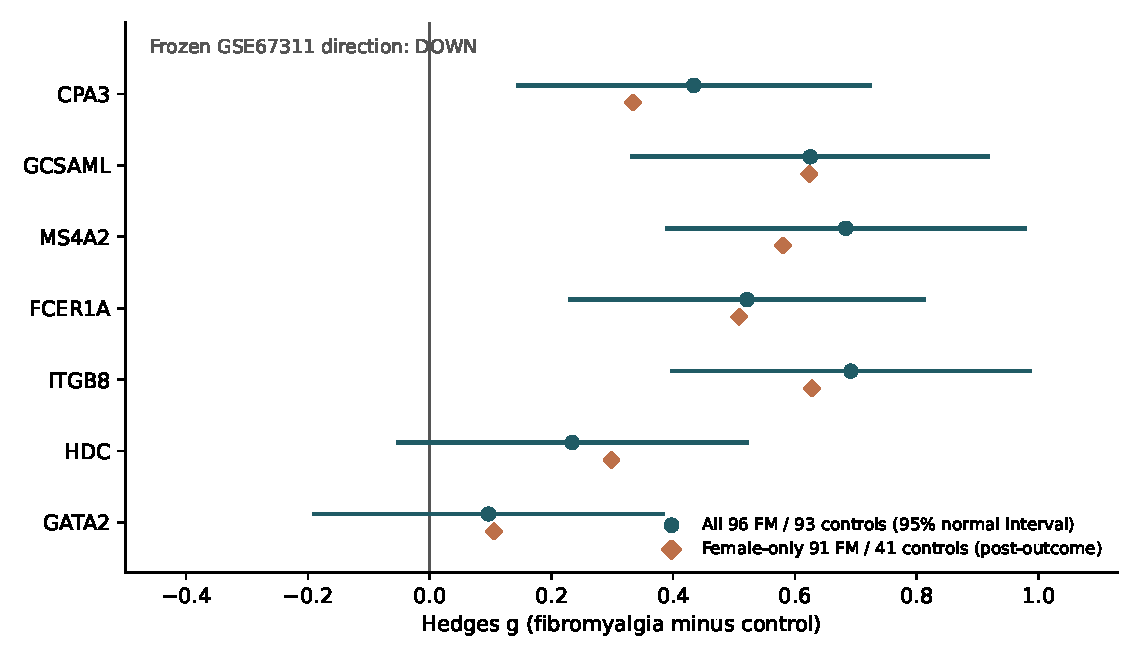
\includegraphics[width=.76\linewidth]{figures/fibromyalgia_p16_effects.pdf}\par\small\refstepcounter{figure}\textbf{Figure \thefigure:} Frozen GSE67311 fibromyalgia DOWN candidates in GSE221921. All seven uniquely measured genes reverse UP. Teal dots and normal-reference intervals show full-cohort Hedges effects; orange diamonds are post-outcome female-only effects. This sensitivity is descriptive, not a new cohort or an opposite-direction biomarker claim. UQCC3 is absent from the unique gene map.\end{center}
The complete P16 sample mapping, effect and sensitivity results are in the repository.

\section{Endometriosis eutopic tissue: a registered panel failure}
After a format-only peek at the count header and first two gene rows, but before calculating cohort-wide effects or inspecting the frozen genes, we fixed twenty discovery-ranked endometriosis genes: seventeen UP and three DOWN. The GEO deposit contains six control eutopic specimens, seven affected-donor eutopic specimens, and seven ectopic specimens (\url{https://www.ncbi.nlm.nih.gov/geo/query/acc.cgi?acc=GSE212787}). Its published multi-omics analysis is at \url{https://doi.org/10.1186/s12967-024-05245-0}. We matched all twenty count column tokens to exact GEO GSM records and sample titles, then used only one primary eutopic count column per each of thirteen distinct donor IDs. Ectopic records from seven affected donors were excluded rather than counted as another validation group; three have paired eutopic and ectopic tissue. The published article describes cohort-one transcriptomic profiling as six control, six eutopic and ten ectopic specimens, whereas the public count matrix maps to six, seven and seven GEO sample records; we cannot reconcile this discrepancy to the published analysis and do not claim a like-for-like published benchmark. An important mapping detail is that a depositor's count token such as NC5P maps to GEO ``patient 13'', not to patient 5. Gene counts, not FPKM columns, were converted to log$_2$(CPM+1); Ensembl IDs with ambiguous HGNC symbol mappings were excluded and remaining duplicate symbols summed before the prespecified CPM filter. Source checksum and full mappings are in \texttt{results/endo\_p17\_*}.

Only ten of the fixed twenty genes were measured by this unambiguous mapping/filter rule, below the registered fifteen-gene minimum. Six of ten measurable signs agree with discovery, versus a 10,000-set direction-preserving, minimum-discovery-coverage null mean of 5.761 and empirical $p=0.5811$; no same-direction gene passes the planned $0.05/20$ nominal family threshold. The registered panel fails on coverage, sign fraction and matched-null probability. The article says participants had normal menstrual cycles and no recent hormone treatment, but GEO metadata do not define menstrual-cycle phase per donor; ``S/P'' file suffixes were not treated as such a definition. This and the published source's prior endometriosis-fibrosis analysis limit any claim of independent biological novelty. The thirteen newly used GSM accessions sit within one GSE, not thirteen independent cohorts. This additional negative leaves the ten-disease tool without a validated endometriosis biomarker.

\section{Another late-placenta six-gene panel failure}
The previously fixed six DOWN preeclampsia genes were tested in historical GSE143953, four placentas with PE and four controls at delivery (\url{https://www.ncbi.nlm.nih.gov/geo/query/acc.cgi?acc=GSE143953}). Workbook columns ECL001/003/004/005 and NEG002/003/004/005 mapped exactly to eight distinct GEO GSM titles and disease labels. The source supplies FPKM rather than integer count values; we used log$_2$(FPKM+1), not a second CPM normalization. The six unambiguous symbol rows are all measured. FES $g=-0.713$ (Welch $p=0.297$), GPAT3 $-0.187$ ($0.773$), FURIN $-0.944$ ($0.215$), GRAMD1A $-0.177$ ($0.790$), ZNF467 $-1.341$ ($0.085$), and LPGAT1 $+0.443$ ($0.512$). Five of six signs agree, not the required six; none has same-direction $p<0.05/6$. The descriptive panel fails. All six effects, source checksum and column-to-GSM mapping are in \texttt{results/pe\_p19\_*}. Eight used GSM records belong to one added GSE; no independent early-pregnancy validation or novel marker follows from this small at-delivery series.

\section{P21 historical severe-PE placenta: fixed-panel descriptive support}
After the six-gene DOWN panel was frozen and had already been examined across many other deposits, GSE148241 offered an at-delivery contrast of nine early-onset severe preeclamptic placentas and 32 recorded normal placentas (\url{https://www.ncbi.nlm.nih.gov/geo/query/acc.cgi?acc=GSE148241}). We registered a diagnostic rule before loading any panel value in this deposit. Two umbilical cord-blood records were excluded. Normal sample titles PHNPR27A/B and PHNPR38A/B may represent repeated tissue from the same donors; the B records were conservatively excluded, leaving 30 controls. Unique donor identity cannot otherwise be established from these titles. Each of the 39 retained GSM raw-count files passed the predeclared integer, nonnegative, common-gene-ID checks. Approved HGNC symbol-to-Ensembl mappings resolved each target once. We computed gene-level $\log_2(\mathrm{CPM}+1)$ and compared case to control with Hedges $g$ and two-sided Welch $p$, using putatively distinct placental specimens rather than genes as the unit of contrast.

All six panel signs point DOWN: FES $g=-2.563$ ($p=0.000663$), GPAT3 $-1.223$ ($p=0.00318$), FURIN $-2.060$ ($p=0.00817$), GRAMD1A $-1.202$ ($p=0.0371$), ZNF467 $-3.193$ ($p=0.000040$) and LPGAT1 $-1.106$ ($p=0.0663$). Four local $p$ values pass $0.05/6$. Thus this deposit meets the registered descriptive six-sign and at-least-one-corrected-gene rule, unlike P19. It does not make any of these genes a newly discovered preeclampsia biomarker: panel choice followed earlier data, the public 2020 deposit is historical, and this contrast is severe PE at delivery rather than prediction at 11--13 weeks or maternal blood. A large effect can reflect gestational age, fetal growth, severity, case mix, or placenta cell composition; the deposit metadata does not resolve those alternatives. The original study investigated RNA-editing dysregulation rather than a prospective version of our six-gene prediction task. Source and sample checksums, all per-gene effects, exact identity mapping and runnable analysis are in \texttt{results/pe\_p21\_*} and \texttt{scripts/pe\_p21\_test.py}. This study contributes one GSE and 39 analyzed GSM records, not 40 independent studies.

\section{P22 preterm-birth comparator: frozen placental panel fails}
The P21 positive contrast used historical early-onset severe PE versus normal placentas at delivery; we then found a different historical study with five early-onset PE and five preterm-birth placentas, GSE177049 (\url{https://www.ncbi.nlm.nih.gov/geo/query/acc.cgi?acc=GSE177049}). This is not a patient-level matched reanalysis of P21, but the preterm-birth comparator makes it a useful, albeit small, test of the frozen six DOWN directions. Before opening any fixed-gene outcome, we registered an all-six-down and at-least-one-corrected-gene descriptive rule. Each of ten workbook RNA sample columns N1--N5 and PE1--PE5 mapped exactly to a disease-labeled GEO RNA GSM; ten corresponding miRNA GSMs were not treated as independent people or counted as gene-expression accessions. The per-sample workbook abundance is FPKM; we used $\log_2(\mathrm{FPKM}+1)$, rather than treating FPKM as a count library.

Three of six signs point DOWN: FES $g=+0.037$ ($p=0.950$), GPAT3 $-0.561$ ($p=0.363$), FURIN $+0.451$ ($p=0.453$), GRAMD1A $+0.438$ ($p=0.471$), ZNF467 $-0.778$ ($p=0.216$), and LPGAT1 $-0.362$ ($p=0.547$). None meets $p<0.05/6$. Thus P22 fails the registered descriptive rule and weakens a broad placental specificity interpretation of P21. Its five-versus-five comparison lacks precision and uses a different study, so it cannot isolate how much of P21's contrast was gestational age, control selection, cell composition or processing. It supplies no early prediction or new discovery. All exact mappings, six effects and workbook checksum are in \texttt{results/pe\_p22\_*}; the original GSE and ten RNA GSMs add eleven used records, not eleven independent cohorts.

\section{P23 gestational-age-matched chorionic-villus panel fails}
A previous generic screen had skipped GSE44711 because its early-onset PE label, \texttt{EOPET}, did not match the parser's case pattern; the series matrix was downloaded, but no case contrast or frozen-panel effect was computed. We reopened only its GEO record and sample metadata, then registered a fixed six-DOWN-gene test before reading any target expression values (\url{https://www.ncbi.nlm.nih.gov/geo/query/acc.cgi?acc=GSE44711}). Its archival 2013 expression subseries contains eight early-onset PE and eight control chorionic-villus arrays on GPL10558, with matched gestational ages claimed by the study. The actual PE gestational weeks span 24.86--37.28; controls span 25.0--36.0. Every title and GSM mapped exactly to a unique matrix column. The source's GSE44712 superseries also includes methylation and does not add independent expression cases.

We applied the committed normalized array transformation and GPL10558 probe-to-symbol mapping, choosing among the two LPGAT1 probes by the global max-mean rule without disease labels. All six frozen targets were measurable. PE minus control Hedges effects and two-sided Welch probabilities are: FES $g=-2.333$, $p=0.000399$; GPAT3 $g=+0.589$, $p=0.2342$; FURIN $g=+0.246$, $p=0.6108$; GRAMD1A $g=-2.256$, $p=0.000939$; ZNF467 $g=-1.406$, $p=0.01141$; LPGAT1 $g=-1.329$, $p=0.01454$. FES and GRAMD1A pass the local $0.05/6$ threshold in the specified direction, but GPAT3 and FURIN reverse, so the registered all-six-DOWN descriptive rule \emph{fails}. The 16 analyzed accessions belong to one old study, not 16 independent validations; we have not individually retrieved their full GSM records for the accession ledger. This gestationally matched contrast cannot repair P21's severity, cell-composition or historical selection bias, and its negative panel result is another limit on broad specificity. Per-GSM ages, source matrix checksum and full effects are in \texttt{results/pe\_p23\_*}. Neither corrected hits nor panel failure establishes a novel biomarker or a clinical predictor.

\section{P24 first-trimester CVS: label-conflicted transport calculation}
GSE295760 is unusually relevant to the originally sought early-pregnancy signal: its chorionic-villus samples were obtained at 11--13 weeks, then linked to later preterm or term preeclampsia (\url{https://www.ncbi.nlm.nih.gov/geo/query/acc.cgi?acc=GSE295760}). After reading only metadata and the non-panel workbook header/first three gene rows, we registered the same six DOWN directions, the primary preterm-PE-versus-control contrast and the complete decision rule. The deposited mRNA RNA-seq metadata and count-workbook columns enumerate four preterm PE, six term PE and nine normotensive controls, while the GEO series description claims four, four and six (14 in all). The linked primary paper reports eighteen collected CVS and fourteen with matched mRNA, small RNA and proteomics used for its DIABLO/LOOCV model (\url{https://pmc.ncbi.nlm.nih.gov/articles/PMC13240503/}). This explains a fourteen-person matched-omics subset, but does not reconcile the eighteen collected specimens with nineteen deposited distinct mRNA titles. We applied the actual nineteen uniquely named mRNA sample columns and their disease-labeled GEO metadata, checked one-to-one mRNA sample tokens, and excluded nineteen small-RNAseq GSMs corresponding to those specimen tokens. A later cross-modality identity audit found four contradictory outcome labels for the same specimen token: C1934 is preterm PE in mRNA but control in small RNA; C1941 is control versus preterm PE; C3729 is term PE versus control; C4144 is control versus term PE. Because the label source cannot be adjudicated, P24 cannot establish even a reliable direction-panel transport outcome. The authors' supplementary material was identified but did not provide a verified token-to-outcome resolution in this analysis. It would be unsound to silently claim that the source-description 14-person design was reproduced. Source workbooks, checksums, exact mappings and both contrasts are in \texttt{results/pe\_p24\_*}.

The 39,533 workbook gene rows were finite nonnegative integer counts in all columns. After full-library $\log_2(\mathrm{CPM}+1)$ normalization, all six uniquely named genes were measurable. In the registered preterm PE (four) versus control (nine) calculation under the mRNA annotations, FES points UP ($g=+0.648$, Welch $p=0.243$) and GPAT3 points UP ($g=+0.336$, $p=0.437$). FURIN ($g=-0.123$, $p=0.750$), GRAMD1A ($g=-0.145$, $p=0.728$), ZNF467 ($g=-0.170$, $p=0.757$) and LPGAT1 ($g=-0.371$, $p=0.426$) point DOWN, with no locally corrected hit. Under the mRNA annotations the six-DOWN and one-$p<0.05/6$ calculation does not pass; the preregistered biological test is \emph{uninterpretable pending identity reconciliation}, not a valid negative replication. The explicitly secondary all-PE (ten versus nine) calculation under the same mRNA metadata retains FES and GPAT3 pointing UP and no corrected hit, but is equally uninterpretable as a disease contrast. Unlike the at-delivery placenta comparisons, these deposited columns represent an early tissue, but the label conflict blocks a valid group test, the sample is small, the deposited mRNA count differs from the paper's collected-specimen count and the already-published multi-omics paper nominated signatures of its own. These label-conflicted measurements do not independently validate or falsify a new named biomarker, furnish a maternal-blood screening assay, or challenge a published benchmark under its own split and endpoint. No new GSMs have been counted in the accession ledger because the identity conflict prevents treating them as validated records; the workbook is one study, not nineteen external validations.

\section{P25 paired Hunner-lesion tissue stress test: fixed IC panel fails}
To test whether the existing interstitial-cystitis discovery signs travel into a more directly diseased bladder specimen, we fixed the original top-fifty gene list, signs, sample mapping and a discovery-sign-matched gene-set null before reading GSE238208 expression values (\url{https://www.ncbi.nlm.nih.gov/geo/query/acc.cgi?acc=GSE238208}). The public historical series supplies paired Hunner lesions and nearby non-lesion mucosa from 25 people with Hunner-type interstitial cystitis, as well as 13 separate BCG-cystitis biopsies. The latter are not healthy controls and were excluded from the registered paired contrast. All 63 FPKM columns in the source workbook map by exact measurement ID to GEO GSM descriptions. Each pair was matched by Case1--Case25 and tissue site; fifty samples represent 25 people. Four fixed genes had no unique measured gene-symbol row, leaving 46 usable genes after discarding duplicate or malformed names.

For each of the 46, we computed the within-person mean lesion-minus-non-lesion $\log_2(\mathrm{FPKM}+1)$ effect and checked its sign against the frozen disease-discovery direction. Only 31/46 agree (67.4\%). Among 10,000 seeded random gene sets preserving the original positive/negative discovery-sign counts and excluding the selected panel, the mean agreement was 55.5\%; empirical one-sided $p=0.0679$. The registered descriptive support condition required at least forty measured, forty matching and $p<0.01$, so it \emph{fails}. Nine of the paired gene tests have nominal $p<0.05$, but zero pass BH correction within the 46-gene measured panel. Exact paired GSM maps, selected gene outcomes, the sampled null, original matrix and expression SHA-256 hashes, and rerunnable code are in \texttt{results/ic\_p25\_*} and \texttt{scripts/ic\_p25\_paired\_transport.py}. The lesion-versus-non-lesion difference is neither patient-level IC diagnosis versus a healthy population nor an independent novelty claim: the published source already studied inflammatory polarization in Hunner lesions. This failure does not disprove all tissue-specific IC signals. It limits this particular panel's proposed transport and is not a published-model benchmark comparison. We did not add these GSMs to the accession manifest without individual full-record verification.

\section{P26 untreated PCOS iPSC-MPC panel: another tissue-shift failure}
The unchanged twenty-gene PCOS discovery panel was registered for a tissue-shift stress test before inspecting target expression in GSE267287 (\url{https://www.ncbi.nlm.nih.gov/geo/query/acc.cgi?acc=GSE267287}). Its published iPSC-derived mesenchymal progenitor cell (MPC) series contains four untreated PCOS-derived and four untreated control-derived cell lines, plus six testosterone-treated samples from some of the same donor-labelled lines. We compared only the eight untreated samples and excluded treated samples rather than inflating independence. GEO titles, disease and treatment characteristics map uniquely to every count header's library description. The count table has 60,715 unique gene-ID rows, including 44 pseudoautosomal \texttt{\_PAR\_Y} Ensembl suffixes; those were mapped by their stable ENSG ID and any coinciding gene symbols summed. Ambiguous HGNC Ensembl mappings were excluded. Gene CPM was based on full-library counts and a filter of CPM greater than one in at least 20\% of primary libraries preceded $\log_2(\mathrm{CPM}+1)$ and effect estimation.

Eighteen of twenty frozen genes passed unique mapping and expression filters. Only ten of eighteen effects share the original discovery direction. In 10,000 seeded direction- and discovery-coverage-matched random panels, the expected count was 8.56 and the empirical one-sided $p=0.3282$. The registered descriptive condition of at least fifteen measurable genes, fifteen agreeing signs and $p<0.025$ therefore \emph{fails}. Full gene-level effects, eight primary versus six excluded GSM mapping, sampled null, checksum-pinned source links and runnable script are in the P26 result ledger and runnable script in the repository. This negative does not overturn the separate small cumulus-cell positive, nor is an induced MPC line interchangeable with ovarian follicular granulosa cells. The historical study already investigated PCOS-associated cell dysfunction; no novel marker, patient-level diagnostic performance or published benchmark superiority follows. These fourteen GSMs were individually fetched and audited in the later P26/P27 accession addendum; the six treated libraries remain excluded from the primary contrast.

\section{P27 full-length granulosa isoform data: fixed PCOS panel fails}
A separate small human granulosa-cell series, GSE294074 (\url{https://www.ncbi.nlm.nih.gov/geo/query/acc.cgi?acc=GSE294074}), deposited six individually named PacBio full-length transcript TPM tables and a functional-annotation table. Its associated paper documents third-generation Iso-Seq and an ovarian energy-metabolism hypothesis (\url{https://pmc.ncbi.nlm.nih.gov/articles/PMC12127534/}). Before opening its target expression, we registered the same twenty discovery-ranked PCOS genes, signs, 10,000 matched-gene null sets and $p<.025$ threshold. The control titles Ctrl-1--3 correspond exactly to GSM8898319--21, and PCOS-1--3 to GSM8898322--24. They are different GSM and SRA accessions from the existing discovery series; nevertheless, participant overlap cannot be ruled out just from accession differences.

We assigned each deposited PB transcript to a gene only when the supplied SwissProt annotation contained a single human \texttt{GN=} symbol. We aggregated its deposited TPM by symbol per specimen and used $\log_2(\mathrm{TPM}+1)$, requiring TPM $>1$ in at least two of six specimens. The six transcript lists have only 2,068 PB identifiers in common and 145,088 in their union. Missing transcript-by-sample entries were zero-filled solely to aggregate the deposited TPM tables; these PB identifiers should not be treated as a shared quantitative transcript universe or proof of biological absence. Five frozen genes did not survive the unique mapping and expression/effect filter: CELA1, LIMCH1, AFAP1L1, F8A3 and ZNF282. Nine of fifteen measurable fixed genes matched the discovery direction; the matched-null mean was 7.2537, empirical one-sided $p=0.2607$. This fails registered descriptive support. The n=3/3 design, isoform annotation and table non-overlap limit any gene-level comparison; a standardized effect as large as MAP7D1 $g=51.56$ reflects unstable tiny-group scaling, not a plausible clinical effect estimate. This adds neither a clinical PCOS biomarker nor a published benchmark win. All twenty gene decisions and 10,000 null draws are retained with the scripts.

\section{P28 cross-parasite leishmaniasis lesion test: the panel fails}
To shift the prospective work beyond PCOS, we locked twenty leishmaniasis genes having at least two original discovery cohorts and BH $q<.05$ before inspecting GSE216638 target expression (\url{https://www.ncbi.nlm.nih.gov/geo/query/acc.cgi?acc=GSE216638}). The associated publication studied \emph{Leishmania tropica} skin lesions (\url{https://www.nature.com/articles/s41598-020-72671-7/}); the historical gene panel derived largely from \emph{L. braziliensis} case-control studies. Exact count-workbook letter columns match the twenty-two GEO specimen-title prefixes and distinct GSMs: seven untreated ulcerative lesions, nine untreated non-ulcerative lesions and six healthy skin controls. Our initial registration incorrectly described an eight/eight ulcerative split; we corrected it in a separate remote commit before expression outcomes, leaving the pooled sixteen-versus-six endpoint unchanged. The supplemental workbook contains both actual integer raw-count columns and already analyzed DE result columns; only the former entered our test. Thirty-three duplicated symbols and one slash-joined annotation were excluded rather than assigned an arbitrary row. We computed $\log_2(\mathrm{CPM}+1)$ with CPM $>1$ in at least 20\% of specimens, then lesion-minus-control Hedges $g$ and Welch tests.

Eighteen frozen genes were measurable; CCL2 and CCR4 were unavailable after unique-mapping/expression filtering. Eleven of eighteen effect signs matched the historical discovery. The 10,000 seeded, direction- and discovery-coverage-matched unselected-gene panels averaged 11.2201 matching signs; one-sided empirical $p=0.6443$. The registered rule of at least fifteen matching signs, fifteen measurable genes, and $p<0.025$ therefore fails. Two measured-panel individual Welch tests pass a within-panel BH correction, PON2 down ($g=-2.614$, $p=1.88\times10^{-7}$, $q=3.38\times10^{-6}$) and CACNA2D2 down ($g=-1.021$, $p=.00333$, $q=.02995$). Those genes were selected after historical disease outcomes and cannot be called fresh discoveries or parasite-specific clinical markers. The failed panel is more informative than spotlighting its two survivors. We preserve all twenty gene outcomes, six controls, sixteen lesion labels, exact source checksums and the sampled null in machine-readable outputs. Different parasite species, specimen mixtures and possible inflammatory confounding prevent a causal reading of concordance or its failure; distinct accession records do not alone prove unrelated participants.

\section{P29 ME/CFS leukocyte-to-plasma cfRNA: panel fails}
Before examining the GSE293840 target matrix (\url{https://www.ncbi.nlm.nih.gov/geo/query/acc.cgi?acc=GSE293840}), we froze all sixteen ME/CFS discovery genes having two original studies and BH $q<.05$, with their historical signs and a direction/coverage-matched 10,000-gene-set null. The new deposit provides plasma cell-free RNA counts from 93 ME/CFS cases and 75 sedentary controls, each mapped to a unique GEO GSM, title subject token and raw-count column token. This is a different assay from the original leukocyte arrays, not a direct technical replication. We mapped version-stripped Ensembl IDs through the project's HGNC reference, excluded ambiguous maps, summed gene counts and calculated $\log_2(\mathrm{CPM}+1)$ after a CPM $>1$ in 20\% filter. Three of the frozen genes (HIST1H3E, PTGER1 and RSG1) failed unique mapping or expression/effect filtering. Only five of the thirteen measurable genes matched the historical direction; the seeded null mean was 6.5439 and one-sided empirical $p=.9490$. The registered rule of at least twelve measurable, twelve matching signs and $p<.025$ fails.

Five measured-panel Welch tests passed within-panel BH $q<.05$, but KCNC3, NEU3 and COQ3 reversed historical direction; only RTF1 and WIPF2 agree. The full per-gene table retains effects, nominal $p$, within-panel $q$, and missingness. Batch-specific matching counts are 6/13, 7/13 and 5/13, site-specific counts 6/13, 6/13 and 4/13, and female/male counts 5/13 and 6/13. These strata each have at least three cases and controls; 104 gene-stratum effects are stored, not screened for a favorable result. The series describes a 0.81 held-out AUC for its own cfRNA classifier, but our sign-transport panel is neither the same model nor its held-out patient split, so no numerical head-to-head or state-of-the-art break follows. The target study was already published, and selection on old outcomes rules out a novel-marker claim from individual target $q$ values alone.

\section{Threats to interpretation and reproducibility contract}
\subsection{Independent study versus independent record}
An accession is an identifier for a data object, not a statistical replicate. We separately list series, sample and platform identifiers in the machine manifest. The 32 individually inspected GSM records were used to verify sample identity and labels but are nested inside eight GSE studies; the explicit \texttt{gsm\_to\_study.csv} map is essential to prevent accidental inflation of the study count. Because a superseries may redeposit the same GSM, we also disallow a GSM in both discovery and held-out validation after the deterministic duplicate audit. The original pre-correction estimates remain in provenance but cannot be used as final validation.

\subsection{Protocol, tissue and phenotype}
A CellxGene human reference dataset of 75,042 normal trophoblast cells from decidua and placenta is catalogued as secondary data, rather than an independent preeclampsia case/control cohort (\url{https://cellxgene.cziscience.com/e/ecf2e08e-2032-4a9e-b466-b65b395f4a02.cxg/}). It illustrates the cell-composition context that bulk placenta mixes; it cannot validate ST3GAL2. Standardizing a within-cohort mean contrast removes measurement scale, not confounding. Different cell fractions, gestational weeks, fertility treatment, blood collection, pooling, medication and array probes can change the sign of a gene's effect. Preeclampsia results illustrate this: ST3GAL2's blood cohort points up while the registered direction was down. The placenta-only sensitivity remains below the decision threshold and is not a replacement for the prespecified four-cohort test. Pooling two patients per library in GSE193123 changes the sampling unit; the variance formula uses three case and three control libraries, not inferred individual measurements.

\subsection{Multiplicity and model-selection boundaries}
The BH formula controls expected false-discovery proportion only under its assumptions for the chosen family; it does not transform a post-hoc shortlist into a registered candidate. The first PCOS exploratory check using a half-probability binomial null looked more promising than the direction-matched null. We retain both numbers, identify the corrected test, and avoid choosing whichever looks favorable. Similarly, a disease panel selected after looking at held-out data would require a new untouched evaluation set. Prediction registration records the accession, feature set, direction, null, threshold and exclusions before processing its expression matrix.

\subsection{Runnable artifacts and audit trail}
The \texttt{ubiomark} Python package exposes reproducible project commands; scripts reconstruct GEO processing, random-effects meta-analysis, graph baselines, CNN evaluation, and figures from local accession downloads and captured annotations. the final split, excluded-series, preregistered-predictions, and per-cohort CSV files record the decisions needed to reproduce negatives as well as positives. Fourteen hermetic tests pass; one tiny-group variance test emits a degrees-of-freedom warning by design. Test passage shows code-path consistency, not external validity or absence of data leakage. Publication requires a fresh clean checkout, pinned sources and complete provenance re-run, and a comparable external benchmark or defensible independently validated discovery; that endpoint is still open.
\section{Limitations of the fixed sign-panel test}
For the P8 PCOS panel, a naive null that each of nineteen measured genes independently agrees with probability one-half would give a deceptively small tail probability for 16 agreements. But the panel was constructed from discovery meta-effects with eighteen positive and one negative direction among the measured set, and those signs are not equiprobable under a cohort-wide shift. The direction- and discovery-coverage-matched null asks a narrower, more honest question: among measured genes with the same direction mix and at least four discovery cohorts, how often does an equally sized random set reach sixteen matches? It does so frequently ($p=0.5884$). The sampled null counts are archived rather than replaced by a fitted theoretical curve. This also warns that a signature's empirical p is conditional on its gene universe and cannot be compared directly with another tissue where the measurable genes differ.

The IC P7 study illustrates a separate limitation. The same urine-sediment cohort includes eight PBS cases, but three have Hunner lesions and five do not. An all-case disease label mixes them; a large lesion-only result on three participants is not a rescue of the all-case failure. The registered primary all-case test returned $p=0.6406$ against its direction-matched gene-set null. The exact post-result reallocation of lesion labels across all 56 possible three-of-eight case partitions yielded two as extreme as the observed lesion-versus-non-lesion contrast. That conditional number describes one historical cohort and selected panel, not an estimate of sensitivity in a future population. The original GEO study already characterized the lesion-specific inflammatory signal; a claim of novelty would be particularly inappropriate. The study also changes specimen from bladder tissue to urine sediment. These two effects are entangled, so the result does not isolate whether tissue or phenotype caused non-transport.

Across diseases, the weak evidence can be mistaken for a strong pattern if the units are blurred: 703 counted accession records are not 703 independent cohorts; ten gene-fold scores are not ten distinct external benchmarks; three pooled libraries per group are not six independent individuals per group; forty-three agreeing genes are not forty-three patients; a null gene-set score is not a clinical AUROC. Each claim should name its observational unit. A future study can falsify this project's fixed panels by preregistering specimen, cell type, phenotype definition, sample mapping, model and threshold, then collecting a patient-level cohort not chosen for a favorable result. Until then, the repository is a reproducible research tool and negative-results account, not a diagnostic product.

\section{Verified primary-literature references}
The following references were checked against DOI-registry titles, journals, and publication dates. The GEO/EBI accession links in the methods and results remain the direct data sources; a paper citation does not convert one cohort into an independent revalidation.
\begin{thebibliography}{99}
\bibitem{10-3389-fimmu-2025-1511529} Zhou, Zhu, Zhang et al.. Identification and validation of immune and diagnostic biomarkers for interstitial cystitis/painful bladder syndrome by integrating bioinformatics and machine-learning. \emph{Frontiers in Immunology}, 2025. DOI: \url{https://doi.org/10.3389/fimmu.2025.1511529}.
\bibitem{10-1371-journal-pone-0161504} Brew, Sullivan, Woodman. Comparison of Normal and Pre-Eclamptic Placental Gene Expression: A Systematic Review with Meta-Analysis. \emph{PLOS ONE}, 2016. DOI: \url{https://doi.org/10.1371/journal.pone.0161504}.
\bibitem{10-1371-journal-pone-0068991} Kleinrouweler, van Uitert, Moerland et al.. Differentially Expressed Genes in the Pre-Eclamptic Placenta: A Systematic Review and Meta-Analysis. \emph{PLoS ONE}, 2013. DOI: \url{https://doi.org/10.1371/journal.pone.0068991}.
\bibitem{10-1186-s13048-025-01956-0} Xu, Zhang, Guo et al.. Interpreting the molecular and cellular landscape of PCOS through bulk transcriptomics, single-cell transcriptomics and machine learning. \emph{Journal of Ovarian Research}, 2026. DOI: \url{https://doi.org/10.1186/s13048-025-01956-0}.
\bibitem{10-1038-s41380-025-03068-z} Björvang, Vrettou, Bujanda Cundin et al.. Differentially expressed transcripts associated with depressive symptoms during pregnancy and postpartum. \emph{Molecular Psychiatry}, 2025. DOI: \url{https://doi.org/10.1038/s41380-025-03068-z}.
\bibitem{10-1093-bioinformatics-btag159} Wei, Sasi, Piepenbrock et al.. KG-Bench: Benchmarking Graph Neural Network Algorithms for Drug Repurposing. \emph{Bioinformatics}, 2026. DOI: \url{https://doi.org/10.1093/bioinformatics/btag159}.
\bibitem{10-1016-j-juro-2011-09-142} Blalock, Korrect, Stromberg et al.. Gene Expression Analysis of Urine Sediment: Evaluation for Potential Noninvasive Markers of Interstitial Cystitis/Bladder Pain Syndrome. \emph{Journal of Urology}, 2012. DOI: \url{https://doi.org/10.1016/j.juro.2011.09.142}.
\bibitem{10-2147-IJWH-S618420} Lin, Tang, Kuang et al.. Peripheral Blood Transcriptomic Features Distinguishing Postpartum Depression from Major Depressive Disorder and Healthy Postpartum Controls. \emph{International Journal of Women's Health}, 2026. DOI: \url{https://doi.org/10.2147/IJWH.S618420}.
\end{thebibliography}


\appendix\section{Accession and tool ledgers}
The distinct scientific tool inventory below is generated from the curated count ledger. It is not a list of every endpoint request, import, or development aid. Any row whose evidence fails inspection must be removed from the gate count. The accession manifest and the sample-to-study map are machine readable; an accession backed by a sample record does not constitute a study-level replicate. The DOI citations checked through Crossref include eight primary papers in the machine-readable bibliography ledger. Direct cohort accession links are kept in the results and source ledgers.
\begin{longtable}{p{3.4cm}p{1.1cm}p{8.6cm}}
\caption{49 distinct counted scientific services or analysis libraries, each with a committed analysis use. Aliases of a service count once and delivery/test/build infrastructure is excluded. Exact evidence paths are in results/program\_tool\_audit.csv.}\\
\hline Scientific tool & Type & Analysis use\\\hline\endfirsthead
\hline Scientific tool & Type & Analysis use\\\hline\endhead
NCBI GEO & service & esearch/esummary/FTP are one GEO service, not separate tools\\
Open Targets Platform & service & Disease-target evidence\\
STRING & service & Human physical PPI\\
PyTorch & library & Neural models\\
scikit-learn & library & Baselines and metrics\\
NumPy & library & Numeric arrays\\
SciPy & library & Sparse graphs and statistics\\
pandas & library & Data tables\\
HGNC & service & Local download and REST same service\\
g:Profiler & service & Enrichment\\
NCBI PubMed & service & Distinct database from GEO\\
Ensembl & service & Gene lookup\\
UniProtKB & service & Protein lookup\\
Europe PMC & service & Literature\\
MyGene.info & service & Identifier cross-check\\
Reactome & service & Pathways\\
ChEMBL & service & Target lookup\\
GTEx Portal & service & Reference gene lookup only\\
Matplotlib & library & Real-data figures\\
QuickGO & service & GO annotation for ST3GAL2\\
IntAct & service & Protein interactions\\
InterPro & service & Protein domain annotations\\
OpenAlex & service & PCOS co-mention literature metadata\\
EMBL-EBI OLS & service & MONDO PCOS exact identifier validation\\
AlphaFold Protein Structure Database & service & Structure prediction metadata for ST3GAL2 and SDC3; not a disease validation\\
EMBL-EBI BioStudies & service & Relevant PE placenta array E-GEOD-4707 checked for early/late onset and pooled reference design; no independent new validation inferred\\
MetaboLights & service & Relevant human PCOS granulosa-cell LC-MS study MTBLS12367 checked; distinct metabolite endpoint does not validate expression sign set\\
CZ CellxGene & service & Human normal trophoblast reference dataset 6963899a used to bound tissue composition; secondary and not a PE disease validation\\
Human Protein Atlas & service & ST3GAL2 protein-evidence and exact Ensembl identifier checked; not clinical validation\\
NCBI ClinVar & service & 105 ST3GAL2 gene-associated records checked to reject inference that candidate lacks clinical variant reports; no preeclampsia link inferred\\
PRIDE Archive & service & Relevant human first-trimester serum PE proteome PXD080843 identified as distinct modality and noncomparable benchmark; prior unrelated query excluded\\
statsmodels & library & Independent Paule-Mandel and DerSimonian-Laird pooled-effect sensitivity for falsified ST3GAL2 preeclampsia prediction\\
NetworkX & library & Physical STRING subgraph components and random edge-count context for fixed PCOS and IC sign panels\\
seaborn & library & Rendered empirical matched-null distributions for PCOS P8 and IC P7 failures using observed draws\\
Crossref & service & Verified titles and publication dates of eight DOI research studies cited in manuscript\\
NHGRI-EBI GWAS Catalog & service & Exact preeclampsia trait MONDO\_0005081 association-gene audit; no independent expression validation inferred\\
RCSB Protein Data Bank & service & Exact human FES kinase structures 8XKP and 3BKB checked for protein/domain context; neither validates a PE biomarker\\
BioGRID & service & Human FES record 108533: 40 interactors and 53 curated interactions with primary interaction pages checked; not PE-specific evidence\\
GlyGen & service & Exact human FES P07332-1 phosphorylation-site records checked to distinguish kinase activity from RNA abundance; no PE mechanism inferred\\
iPTMnet & service & Exact FES P07332 kinase-substrate entry checked BCR Y177 and PECAM1 Y690 to separate PTM mechanism from RNA; source overlap and no PE relevance stated\\
WikiPathways & service & Current human pathway-node exact-symbol audit of six frozen P9 genes; no PE disease validation or independent assay inferred\\
Monarch Initiative & service & Resolved exact PE MONDO ID to phenotype and three direct Orphanet-derived associated genes; six-gene fixed-panel absence is resource-specific, not evidence of novelty\\
Human Cell Atlas Data Portal & service & Exact PE PBMC project source screened via Azul index: five donors, 80,429 estimated cells, pregnancy/postpartum context; not counted as independently validated expression\\
TISSUES (JensenLab) & service & Fetched 339455 human curated tissue-evidence rows and checked six frozen PE genes at exact blood/placenta tissues; one FURIN blood record is context only\\
EMBL-EBI BioSamples & service & Verified cross-archive GSM8158605/SAMN40568562/SRS20810958 identity and repeated T-title vs PE-group conflict; mirrored depositor fields do not adjudicate label\\
EMBL-EBI ENA Portal & service & Mapped conflicted P45 BioSample to exactly one RNA-Seq run SRR28411428 and project PRJNA1090471; run identity, not diagnosis or expression validation\\
KEGG REST & service & Mapped pinned HGNC Entrez IDs for six fixed PE genes to KEGG human pathways; cross-resource pathway disagreement contextualized, not evidence of PE validation\\
Human Phenotype Ontology & service & Fetched versioned 2026-09-02 HPO annotations and exact disease-name PE entries; excluded falsely assumed OMIM ID after row audit; phenotype context only\\
BindingDB & service & Exact FES UniProt P07332 query returned 53 heterogeneous ligand-affinity records; druggability context only, no PE efficacy or peptide validation\\
\hline\end{longtable}

 \end{document}
